\documentclass[12pt]{SolutionManual}

\usepackage{mypackages} % put your packages in the file mypackages.sty
\usepackage{mycommands} % put your commands in the file mycommands.sty

\def \authorName{P.O. Bolduc} % name of the author

% Some books have two titles (if not just put in \mainTitle)
\def \firstTitle{Volume 1 of Course of Theoretical Physics}
\def \mainTitle{Mechanics}

\begin{document}

\maketitle % insert title page
\tableofcontents % insert table of content

% Put the solutions of each chapter in separate files and use \input{}
\chapter{The Equations of Motion}

% ============ Problem 1 ============ %

\begin{problem}
{
Find the Lagrangian of a coplanar double pendulum when placed in a uniform gravitational field (acceleration $g$).
\begin{figure}[H]
    \centering
    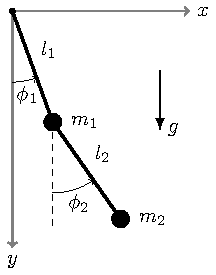
\includegraphics[page=1]{Figures/tikzpics.pdf}
\end{figure}
}
{
The generalized co-ordinates of the system are the two angles $\phi_1$ and $\phi_2$. We need to express the Cartesian co-ordinates in terms of those two angles. First, the Cartesian position of the particle $m_1$ is
\begin{align*}
    x_1 &= f_1(\phi_1) = l_1 \sin{\phi_1} \\
    y_1 &= g_1(\phi_1) = l_1 \cos{\phi_1} .
\end{align*}
By taking the time derivative of those, we obtain
\begin{align*}
    \Dot{x}_1 &= \pd{f_1}{\phi_1} \Dot{\phi}_1 = l_1 \cos{\phi_1} \Dot{\phi}_1 \\
    \Dot{y}_1 &= \pd{g_1}{\phi_1}\Dot{\phi}_1 = -l_1 \sin{\phi_1} \Dot{\phi}_1 .
\end{align*}
Substituting these expressions in the Lagrangian, we obtain the desired Lagrangian form, that is
\begin{align*}
    L_1 &= T_1 - U_1 \\
    &= \frac{1}{2} m_1 (\Dot{x}_1^2 + \Dot{y}_1^2) + m_1 g y_1 \\
    &= \frac{1}{2} m_1 l_1^2 \Dot{\phi}_1^2 + m_1 g l_1 \cos{\phi_1} . \numberthis \label{C1P1_L1}
\end{align*}
Second, the Cartesian position of the particle $m_2$ is
\begin{align*}
    x_2 &= f_2(\phi_1, \phi_2) = l_1 \sin{\phi_1} + l_2 \sin{\phi_2} \\
    y_2 &= g_2(\phi_1, \phi_2) = l_1 \cos{\phi_1} + l_2 \cos{\phi_2} .
\end{align*}
By taking the time derivative of those, we obtain
\begin{align*}
    \Dot{x}_2 &= \sum_k \pd{f_2}{\phi_k} \Dot{\phi}_k = l_1 \Dot{\phi}_1 \cos{\phi_1} + l_2 \Dot{\phi}_2 \cos{\phi_2} \\
    \Dot{y}_2 &= \sum_k \pd{g_2}{\phi_k} \Dot{\phi}_k = -l_1 \Dot{\phi}_1 \sin{\phi_1} -l_2 \Dot{\phi}_2 \sin{\phi_2} .
\end{align*}
Substituting these expressions in the Lagrangian, we obtain the desired Lagrangian form, that is
\begin{align*}
    L_2 &= T_2 - U_2 \\
    &= \frac{1}{2} m_2 (\Dot{x}_2^2 + \Dot{y}_2^2) + m_2 g y_2 \\
    &= \frac{1}{2} m_2 (l_1^2\Dot{\phi}_1^2 + l_2^2\Dot{\phi}_2^2 + 2l_1l_2\Dot{\phi}_1\Dot{\phi}_2\cos{(\phi_1 - \phi_2)}) + m_2 g (l_1 \cos{\phi_1} + l_2 \cos{\phi_2}) , \numberthis \label{C1P1_L2}
\end{align*}
where the angle difference identity as been used. Finally, the Lagrangian of the complete system is simply the sum of \eqref{C1P1_L1} and \eqref{C1P1_L2}, thus
}
{
\begin{align*}
    L = &\frac{1}{2}(m_1+m_2)l_1^2\Dot{\phi}_1^2 + \frac{1}{2}m_2l_2^2\Dot{\phi}_2^2 + m_2l_1l_2\Dot{\phi}_1\Dot{\phi}_2\cos{(\phi_1-\phi_2)} \\
    &+ (m_1+m_2)gl_1\cos{\phi_1} + m_2gl_2\cos{\phi_2}
\end{align*}
}
\end{problem}

% ============ Problem 2 ============ %

\begin{problem}
{
Find the Lagrangian of a simple pendulum of mass $m_2$, with a mass $m_1$ at the point of support which can move on a horizontal line lying in the plane in which $m_2$ moves when placed in a uniform gravitational field (acceleration $g$).
\begin{figure}[H]
    \centering
    \includegraphics[page=2]{Figures/tikzpics.pdf}
\end{figure}
}
{
The generalized co-ordinates $q$ of the system are the position $x$ and the angle $\phi$. Therefore, the Lagrangian of the first particle is simply
\begin{equation}
    L_1 = T_1 = \frac{1}{2} m_1 \Dot{x}^2. \label{C1P2_L1}
\end{equation}
The Cartesian position of the particle $m_2$ can be express in terms of the generalized co-ordinates by
\begin{align*}
    x_2 &= f_2(x, \phi) = x + l \sin{\phi} \\
    y_2 &= g_2(x, \phi) = l \cos{\phi} .
\end{align*}
The time derivative of the position is then
\begin{align*}
    \Dot{x}_2 &= \sum_k \pd{f_2}{q_k} \Dot{q}_k = \Dot{x} + l \Dot{\phi} \cos{\phi} \\
    \Dot{y}_2 &= \sum_k \pd{g_2}{q_k} \Dot{q}_k = - l \Dot{\phi} \sin{\phi} .
\end{align*}
\begin{align*}
    L_2 &= T_2 - U_2 \\
    &= \frac{1}{2} m_2 (\Dot{x}_2^2 + \Dot{y}_2^2) + m_2 g y_2 \\
    &= \frac{1}{2} m_2 (\Dot{x}^2 + l^2 \Dot{\phi}^2 + 2 l \Dot{x} \Dot{\phi} \cos{\phi}) + m_2 g l \cos{\phi} . \numberthis \label{C1P2_L2}
\end{align*}
Finally, the Lagrangian of the complete system is the sum of the two Lagrangian \eqref{C1P2_L1} and \eqref{C1P2_L2}, thus
}
{
\begin{equation*}
    L = \frac{1}{2} (m_1 + m_2) \Dot{x}^2 +  \frac{1}{2} m_2 (l^2 \Dot{\phi}^2 + 2 l \Dot{x} \Dot{\phi} \cos{\phi} ) + m_2 g l \cos{\phi}
\end{equation*}
}
\end{problem}

% ============ Problem 3 ============ %

\begin{problem} 
{
Find the Lagrangian of a simple pendulum of mass $m$, when placed in a uniform gravitational field (acceleration $g$), whose point of support ...
\begin{figure}[H]
    \centering
    \includegraphics[page=3]{Figures/tikzpics.pdf}
\end{figure}
}{}{}
\end{problem}
\begin{subproblem}
{
moves uniformly on a vertical circle with constant frequency $\gamma$.
}
{
If we set that the rotation of the point of support is counterclockwise, the Cartesian position of the particle $m$ is
\begin{align*}
    x &= f(\phi_1) = a \cos{\gamma t} + l \sin{\phi} \\
    y &= g(\phi_1) = -a \sin{\gamma t} + l \cos{\phi} .
\end{align*}
The time derivative of the position is then
\begin{align*}
    \Dot{x} &= -a \gamma \sin{\gamma t} + l \Dot{\phi} \cos{\phi} \\
    \Dot{y} &= -a \gamma \cos{\gamma t} - l \Dot{\phi} \sin{\phi} .
\end{align*}
The potential energy of the system is 
\begin{align*}
    U &= -mgy \\
    &= -mg(-a \sin{\gamma t} + l \cos{\phi}).
\end{align*}
The term $mga \sin{\gamma t}$ only depend on time and can therefore be ignored (does not contribute to the equations of motion). The kinetic energy of the particle, for its part, is
\begin{align*}
    T &= \frac{1}{2} m (\Dot{x}^2 + \Dot{y}^2)\\
    &= \frac{1}{2} m \left(l^2\Dot{\phi}^2 + a^2\gamma^2 +2a\gamma l \Dot{\phi}\sin{(\phi - \gamma t)}\right),
\end{align*}
using again the angle difference identity (I will stop mentioning it). We can observe that the term $\frac{1}{2}ma^2\gamma^2$ is a constant, thus can be ignored. The last term of the kinetic energy can also be simplified. Indeed, 
\begin{align*}
      m a\gamma l \Dot{\phi}\sin{(\phi - \gamma t)} &= m a l \gamma (\dot{\phi} - \gamma) \sin(\phi - \gamma t) + m a l \gamma^2 \sin(\gamma t - \phi) \\
     &= \frac{d}{dt} \left(-m a l  \gamma \cos(\phi - \gamma t) \right) + m a l  \gamma^2 \sin(\phi - \gamma t) .
\end{align*}
After dropping the total time derivative, we can finally get the Lagrangian
}
{
\begin{equation*}
    L = \frac{1}{2} m l^2\Dot{\phi}^2 + m a l  \gamma^2 \sin(\phi - \gamma t)  + mgl\cos{\phi}
\end{equation*}
}
\end{subproblem}

\begin{subproblem}
{
oscillates horizontally in the plane of motion of the pendulum according to the law $x=a\cos{\gamma t}$.
}
{
The Cartesian position of the particle $m$ is
\begin{align*}
    x &= f(\phi_1) = a \cos{\gamma t} + l \sin{\phi} \\
    y &= g(\phi_1) = l \cos{\phi} .
\end{align*}
The time derivative of the position is then
\begin{align*}
    \Dot{x} &= -a \gamma \sin{\gamma t} + l \Dot{\phi} \cos{\phi} \\
    \Dot{y} &= - l \Dot{\phi} \sin{\phi} .
\end{align*}
The potential energy of the system is 
\begin{equation*}
    U = -mgy = -mgl\cos{\phi},
\end{equation*}
and the kinetic energy
\begin{align*}
    T &= \frac{1}{2} m (\Dot{x}^2 + \Dot{y}^2)\\
    &= \frac{1}{2} m \left(l^2\Dot{\phi}^2 + a^2\gamma^2\sin^2{\gamma t} - 2a\gamma l \Dot{\phi}\sin{\gamma t}\cos{\phi}\right).
\end{align*}
We first see that the term $\frac{1}{2} m a^2\gamma^2\sin^2{\gamma t}$ only depend on time. The last term of the kinetic energy can also be simplified. Indeed, 
\begin{align*}
      - m a\gamma l \Dot{\phi}\sin{\gamma t}\cos{\phi} &= 
      -m l a \gamma (\gamma \cos{\gamma t} \sin{\phi} + \Dot{\phi} \sin{\gamma t}\cos{\phi}) + m l a \gamma^2 \cos{\gamma t}\sin{\phi} \\
      &= \frac{d}{dt} \left( -mla\gamma\sin{\gamma t}\sin{\phi} \right) + m l a \gamma^2 \cos{\gamma t}\sin{\phi}.
\end{align*}
After dropping the total time derivative, we can finally get the Lagrangian
}
{
\begin{equation*}
    L = \frac{1}{2} m l^2\Dot{\phi}^2 + m l a \gamma^2 \cos{\gamma t}\sin{\phi}  + mgl\cos{\phi}
\end{equation*}
}
\end{subproblem}

\begin{subproblem}
{
 oscillates vertically according to the law $y=a\cos{\gamma t}$.
}
{
The Cartesian position of the particle $m$ is
\begin{align*}
    x &= f(\phi_1) = l \sin{\phi} \\
    y &= g(\phi_1) = a \cos{\gamma t} + l \cos{\phi} .
\end{align*}
The time derivative of the position is then
\begin{align*}
    \Dot{x} &= l \Dot{\phi} \cos{\phi} \\
    \Dot{y} &= -a \gamma \sin{\gamma t} - l \Dot{\phi} \sin{\phi} .
\end{align*}
The potential energy of the system is 
\begin{equation*}
    U = -mgy = -mg \left( a \cos{\gamma t} + l \cos{\phi} \right),
\end{equation*}
The term $mga \cos{\gamma t}$ only depend on time and can therefore be ignored. The kinetic energy is
\begin{align*}
    T &= \frac{1}{2} m (\Dot{x}^2 + \Dot{y}^2)\\
    &= \frac{1}{2} m \left(l^2\Dot{\phi}^2 + a^2\gamma^2\sin^2{\gamma t} + 2a\gamma l \Dot{\phi}\sin{\gamma t}\sin{\phi}\right).
\end{align*}
We first see that the term $\frac{1}{2} m a^2\gamma^2\sin^2{\gamma t}$ only depend on time. The last term of the kinetic energy can also be simplified. Indeed, 
\begin{align*}
       m a\gamma l \Dot{\phi}\sin{\gamma t}\sin{\phi} &= 
      m l a \gamma (-\gamma \cos{\gamma t} \cos{\phi} + \Dot{\phi} \sin{\gamma t}\sin{\phi}) + m l a \gamma^2 \cos{\gamma t}\cos{\phi} \\
      &= \frac{d}{dt} \left( mla\gamma\cos{\gamma t}\sin{\phi} \right) + m l a \gamma^2 \cos{\gamma t}\cos{\phi}.
\end{align*}
After dropping the total time derivative, we can finally get the Lagrangian
}
{
\begin{equation*}
    L = \frac{1}{2} m l^2\Dot{\phi}^2 + m l a \gamma^2 \cos{\gamma t}\cos{\phi}  + mgl\cos{\phi}
\end{equation*}
}
\end{subproblem}

% ============ Problem 4 ============ %

\begin{problem}
{
Find the Lagrangian of a simple pendulum of the system below when placed in a uniform gravitational field (acceleration $g$). The particle $m_2$ moves on a vertical axis and the whole system rotates about this axis with a constant angular velocity~$\Omega$.
\begin{figure}[H]
    \centering
    \includegraphics[page=4]{Figures/tikzpics.pdf}
\end{figure}
}
{
The position of each particle $m_1$ is best described in cylindrical coordinates, which is
\begin{align*}
    r_1 &= a \sin{\theta} \\
    \phi_1 &= \phi \\
    z_1 &= a \cos{\theta},
\end{align*}
where $\phi$ is the angle of rotation of the system about the axis; $\Dot{\phi} = \Omega$. The kinetic energy of each particle $m_1$ is thus
\begin{align*}
    T_1 &= \frac{1}{2} m_1 ( \Dot{r}_1^2 + r_1^2\Dot{\phi}_1^2 + \Dot{z}_1^2 ) \\
    &= \frac{1}{2} m_1 ( a^2\Dot{\theta}^2\cos^2{\theta} + a^2\Omega^2\sin^2{\theta} + a^2\Dot{\theta}^2\sin^2{\theta} ) \\
    &= \frac{1}{2} m_1 a^2 ( \Dot{\theta}^2 + \Omega^2\sin^2{\theta} ) . \numberthis \label{C1P4_T1}
\end{align*}
The potential energy of this particle can be found by using the $z$ component of his position, namely
\begin{align*}
    V_1 &= -m_1gz_1 \\
    &= -m_1ga\cos{\theta}. \numberthis \label{C1P4_V1}
\end{align*}
The particle $m_2$, in its case, can only move up and down, thus its position can be completely defined by
\begin{equation*}
    z_2 = 2 a \cos{\theta}.
\end{equation*}
Then, the kinetic energy of each particle $m_2$ is
\begin{align*}
    T_2 &= \frac{1}{2} m_2 \Dot{z}_2^2 \\
    &= m_2 a^2 \Dot{\theta}^2 \sin^2{\theta} \numberthis \label{C1P4_T2}
\end{align*}
and the potential energy is
\begin{align*}
    V_2 &= - m_2 g z_2 \\
    &= - 2 m_2 g a \cos{\theta}. \numberthis \label{C1P4_V2}
\end{align*}
Using \eqref{C1P4_T1}, \eqref{C1P4_V1}, \eqref{C1P4_T2} and \eqref{C1P4_V2}, the Lagrangian of the system is
\begin{equation*}
    L = 2(T_1 + T_2 - V_1 - V_2),
\end{equation*}
therefore
}
{
\begin{equation*}
    L = m_1 a^2 ( \Dot{\theta}^2 + \Omega^2\sin^2{\theta} ) + 2m_2 a^2 \Dot{\theta}^2 \sin^2{\theta} + 2(m_1+2m_2)ga\cos{\theta}
\end{equation*}
}
\end{problem}
\chapter{Conservation Laws}

% ============ Problem 1 ============ %

\begin{problem}
{
A particle of mass $m$ moving with velocity $\mathbf{v}_1$ leaves a half-space in which its potential energy is a constant $U_1$ and enters another in which its potential energy is a different constant $U_2$. Determine the change in the direction of motion of the particle.
}
{
The potential energy only depend on the co-ordinate perpendicular to the plane separating the half-space. Thus, the component of the momentum in that plane is conserved. Denoting by $\theta_1$ and $\theta_2$ the angles between the normal to the plane and the velocities $v_1$ and $v_2$ of the particle before and after passing the plane, we have
\begin{align*}
    & P_1 \sin{\theta_1} = P_2 \sin{\theta_2} \\
    \Rightarrow & v_1 \sin{\theta_1} = v_2 \sin{\theta_2} \\
    \Rightarrow & \frac{\sin{\theta_1}}{\sin{\theta_2}} = \frac{v_2}{v_1} . \numberthis \label{C2P1_P}
\end{align*}
The potential energy of the system is also independent of time, therefore the energy of the particle is conserved. Posing $E_1 = T_1 + U_1$ and $E_2 = T_2 + U_2$ as the energy of the particle before and after passing the plane, the law of conservation of energy requires
\begin{align*}
    &E_1 = E_2 \\
    \Rightarrow & T_1 + U_1 = T_2 + U_2 \\
    \Rightarrow &\frac{1}{2} m v_1^2 + U_1 = \frac{1}{2} m v_2^2 + U_2 \\
    \Rightarrow & v_2^2 = v_1^2 + \frac{2}{m}(U_1-U_2). \numberthis \label{C2P1_E}
\end{align*}
By substituting \eqref{C2P1_E} in the square of \eqref{C2P1_P}, we get
\begin{equation*}
    \left( \frac{\sin{\theta_1}}{\sin{\theta_2}} \right)^2 = \frac{v_1^2 + \frac{2}{m}(U_1-U_2)}{v_1^2}.
\end{equation*}
After taking the square root, the result is  
}
{
\begin{equation*}
    \frac{\sin{\theta_1}}{\sin{\theta_2}} = \sqrt{1 + \frac{2}{mv_1^2}(U_1-U_2)}
\end{equation*}
}
\end{problem}

% ============ Problem 2 ============ %

\begin{problem}
{
Find the law of transformation of the action $S$ from one inertial frame to another.
}
{
The Lagrangian $L$ and $L'$ of a mechanical system in two inertial frames of reference $K$ and $K'$ are respectively
\begin{equation*}
    L = T - U = \frac{1}{2} \sum_a m_a v_a^2 - U
\end{equation*}
and
\begin{equation*}
    L' = T' - U = \frac{1}{2} \sum_a m_a v_a^{'2} - U.
\end{equation*}
If the frame $K'$ moves with velocity $\mathbf{V}$ relative to the frame $K$, the velocities of the particles of the mechanical system relative to the two frames are related by $\mathbf{v}_a = \mathbf{v}_a' + \mathbf{V}$. We can now express the relation of the Lagrangian of the system in the two frames by
\begin{align*}
    L &= \frac{1}{2} \sum_a m_a (\mathbf{v}_a' + \mathbf{V})^2 - U \\ 
    &= \frac{1}{2} V^2 \sum_a m_a + \mathbf{V} \cdot \sum_a m_a \mathbf{v}_a' + \frac{1}{2} \sum_a m_a v_a^{'2} - U \\
    &= L' + \mathbf{V} \cdot \mathbf{P}' + \frac{1}{2} \mu V^2 . \numberthis \label{C3P2_L}
\end{align*}
Integrating \eqref{C3P2_L} with respect to time, we obtain
\begin{align*}
    S &= \int L dt \\
    &= S' + \int \left( \mathbf{V} \cdot \mathbf{P}' \right)dt + \frac{1}{2} \mu V^2 t \\
    &= S' + \mathbf{V} \cdot \int \sum_a m_a \mathbf{v}_a' dt + \frac{1}{2} \mu V^2 t \\
    &= S' + \mathbf{V} \cdot \sum_a m_a \mathbf{r}_a' + \frac{1}{2} \mu V^2 t .
\end{align*}
The law of transformation of the action $S$ is then
}
{
\begin{equation*}
    S = S' + \mu \mathbf{V} \cdot \mathbf{R}' + \frac{1}{2} \mu V^2 t
\end{equation*}
}
\end{problem}

% ============ Problem 3 ============ %

\begin{problem}
{
Obtain the expressions for the Cartesian components and the magnitude of the angular momentum of a particle in cylindrical co-ordinates $r,\phi,z$.
}
{
The Cartesian components of the angular momentum are simply
\begin{equation*}
    \mathbf{M} = \mathbf{r} \times \mathbf{p} = \begin{bmatrix} x \\ y \\ z \end{bmatrix} \times m \begin{bmatrix} \Dot{x} \\ \Dot{y} \\ \Dot{z} \end{bmatrix} = m \begin{bmatrix} y \Dot{z} - z \Dot{y} \\ z \Dot{x} - x \Dot{z} \\ x \Dot{y} - y \Dot{x} \end{bmatrix} . \numberthis \label{C3P3_M}
\end{equation*}
In cylindrical co-ordinates, the Cartesian components are expressed by
\begin{equation*}
    \begin{bmatrix} x \\ y \\ z \end{bmatrix} = \begin{bmatrix} r \cos{\phi} \\ r \sin{\phi} \\ z \end{bmatrix}
\end{equation*}
and
\begin{equation*}
    \begin{bmatrix} \Dot{x} \\ \Dot{y} \\ \Dot{z} \end{bmatrix} = \begin{bmatrix} \Dot{r}\cos{\phi} - r\Dot{\phi}\sin{\phi} \\ \Dot{r}\sin{\phi} + r\Dot{\phi}\cos{\phi} \\ \Dot{z} \end{bmatrix}.
\end{equation*}
By substituting those in \eqref{C3P3_M}, we get
\begin{align*}
    \mathbf{M} &= m \begin{bmatrix} y \Dot{z} - z \Dot{y} \\ z \Dot{x} - x \Dot{z} \\ x \Dot{y} - y \Dot{x} \end{bmatrix} \\
    &= m \begin{bmatrix} (r\Dot{z} - z\Dot{r})\sin{\phi} - rz\Dot{\phi}\cos{\phi} \\ -(r\Dot{z} - z\Dot{r})\cos{\phi} - rz\Dot{\phi}\sin{\phi} \\ r^2\Dot{\phi} \end{bmatrix} . \numberthis \label{C3P3_M2}
\end{align*}
By taking the magnitude of \eqref{C3P3_M2}, we finally get
}
{
\begin{align*}
    M_x &= m(r\Dot{z} - z\Dot{r})\sin{\phi} - mrz\Dot{\phi}\cos{\phi} \\
    M_y &= -m(r\Dot{z} - z\Dot{r})\cos{\phi} - mrz\Dot{\phi}\sin{\phi} \\
    M_z &= mr^2\Dot{\phi} \\
    M^2 &= m^2r^2\Dot{\phi}^2(r^2 + z^2) + m^2(r\Dot{z} - z\Dot{r})^2
\end{align*}
}
\end{problem}

% ============ Problem 4 ============ %

\begin{problem}
{
Obtain the expressions for the Cartesian components and the magnitude of the angular momentum of a particle in spherical co-ordinates $r,\theta,\phi$.
}
{
In spherical co-ordinates, the Cartesian components are expressed by
\begin{equation*}
    \begin{bmatrix} x \\ y \\ z \end{bmatrix} = \begin{bmatrix} r \sin{\phi} \cos{\theta} \\ r \sin{\phi} \sin{\theta} \\ r \cos{\phi} \end{bmatrix}
\end{equation*}
and
\begin{equation*}
    \begin{bmatrix} \Dot{x} \\ \Dot{y} \\ \Dot{z} \end{bmatrix} = \begin{bmatrix} \Dot{r}\sin{\phi}\cos{\theta} + r\Dot{\phi}\cos{\phi}\cos{\theta} - r\Dot{\theta}\sin{\phi}\sin{\theta} \\ \Dot{r}\sin{\phi}\sin{\theta} + r\Dot{\phi}\cos{\phi}\sin{\theta} + r\Dot{\theta}\sin{\phi}\cos{\theta} \\ \Dot{r}\cos{\phi} + r\sin{\phi} \end{bmatrix}.
\end{equation*}
By substituting those in \eqref{C3P3_M}, we get
\begin{align*}
    \mathbf{M} &= m \begin{bmatrix} y \Dot{z} - z \Dot{y} \\ z \Dot{x} - x \Dot{z} \\ x \Dot{y} - y \Dot{x} \end{bmatrix} \\
    &= m \begin{bmatrix} -r^2(\Dot{\theta}\sin{\phi} + \Dot{\phi}\sin{\theta}\cos{\theta}\cos{\phi}) \\ r^2(\Dot{\theta}\cos{\phi} - \Dot{\phi}\sin{\theta}\cos{\theta}\sin{\phi}) \\ r^2\Dot{\phi}\sin^2{\theta} \end{bmatrix} . \numberthis \label{C3P3_M3}
\end{align*}
By taking the magnitude of \eqref{C3P3_M3}, we finally get
}
{
\begin{align*}
    M_x &= -mr^2(\Dot{\theta}\sin{\phi} + \Dot{\phi}\sin{\theta}\cos{\theta}\cos{\phi}) \\
    M_y &= mr^2(\Dot{\theta}\cos{\phi} - \Dot{\phi}\sin{\theta}\cos{\theta}\sin{\phi}) \\
    M_z &= mr^2\Dot{\phi}\sin^2{\theta} \\
    M^2 &= m^2r^4(\Dot{\theta}^2 + \Dot{\phi}^2\sin^2{\theta})
\end{align*}
}
\end{problem}

% ============ Problem 5 ============ %

\begin{problem}
{
Which components of momentum $\mathbf{P}$ and angular momentum $\mathbf{M}$ are conserved in motion in the following fields ?
}{}{}
\end{problem}
\begin{subproblem}
{
The field of an infinite homogeneous plane.
}
{
solution
\begin{figure}[H]
    \centering
    \includegraphics[page=5]{Figures/tikzpics.pdf}
\end{figure}
}
{
answer
}
\end{subproblem}

\begin{subproblem}
{
The field of an infinite homogeneous cylinder.
}
{
solution
}
{
answer
}
\end{subproblem}

\begin{subproblem}
{
The field of an infinite homogeneous prism.
}
{
solution
}
{
answer
}
\end{subproblem}

\begin{subproblem}
{
The field of two points.
}
{
solution
}
{
answer
}
\end{subproblem}

\begin{subproblem}
{
The field of an infinite homogeneous half-plane.
}
{
solution
}
{
answer
}
\end{subproblem}

\begin{subproblem}
{
The field of a homogeneous cone.
}
{
solution
}
{
answer
}
\end{subproblem}

\begin{subproblem}
{
The field of a homogeneous circular torus.
}
{
solution
}
{
answer
}
\end{subproblem}

\begin{subproblem}
{
The field of an infinite homogeneous cylindrical helix.
}
{
solution
}
{
answer
}
\end{subproblem}

% ============ Problem 6 ============ %

\begin{problem}
{
Find the ratio of the times in the same path for particles having different masses but the same potential energy.
}
{
If the two particles have the same path, then the ratio of linear dimension is
\begin{equation} \label{C3P1_l}
    \frac{l'}{l} = \alpha = 1.
\end{equation}
We can define the ratio of time and mass by
\begin{equation*}
    \frac{t'}{t} = \beta
\end{equation*}
and
\begin{equation*}
    \frac{m'}{m} = \gamma .
\end{equation*}
Then, the ratio of kinetic energy is 
\begin{equation*}
    \frac{T'}{T} = \frac{m' \mathbf{v}'}{m \mathbf{v}} = \frac{m'}{m} \left( \frac{\mathbf{dr}'}{\mathbf{dr}} \frac{dt}{dt'} \right)^2 = \frac{\gamma \alpha^2}{\beta^2}.
\end{equation*}
To leave the equation of motion unaltered, the ratio of the kinetic energy and the potential energy must be the same, \ie,
\begin{align*}
    \frac{U'}{U} &= \frac{T'}{T} \\
    \Rightarrow \alpha^k &=  \frac{\gamma \alpha^2}{\beta^2}.
\end{align*}
Using \eqref{C3P1_l}, we get
\begin{align*}
    1 &= \frac{\gamma}{\beta^2} \\
    \Rightarrow \beta &= \sqrt{\gamma}.
\end{align*}
The ratio of the times is then
}
{
\begin{equation*}
    \frac{t'}{t} = \sqrt{\frac{m'}{m}}
\end{equation*}
}
\end{problem}

% ============ Problem 7 ============ %

\begin{problem}
{
Find the ratio of the times in the same path for particles the same mass but potential energy differing by a constant factor.
}
{
If the two particles have the same path, then the ratio of linear dimension is
\begin{equation} \label{C3P2_l}
    \frac{l'}{l} = \alpha = 1.
\end{equation}
We can define the ratio of time by
\begin{equation*}
    \frac{t'}{t} = \beta .
\end{equation*}
Then, the ratio of kinetic energy is 
\begin{equation*}
    \frac{T'}{T} = \frac{\alpha^2}{\beta^2}.
\end{equation*}
The potential energy of the two particles differ by a constant factor, which mean that
\begin{equation*}
    \frac{U'}{U} = \gamma .
\end{equation*}
To leave the equation of motion unaltered, the ratio of the kinetic energy and the potential energy must be the same, \ie,
\begin{align*}
    \frac{U'}{U} &= \frac{T'}{T} \\
    \Rightarrow \gamma &=  \frac{\alpha^2}{\beta^2}.
\end{align*}
Using \eqref{C3P2_l}, we get
\begin{align*}
    \gamma &= \frac{1}{\beta^2} \\
    \Rightarrow \beta &= \sqrt{\frac{1}{\gamma}}.
\end{align*}
The ratio of the times is then
}
{
\begin{equation*}
    \frac{t'}{t} = \sqrt{\frac{U}{U'}}
\end{equation*}
}
\end{problem}
\chapter{Integration of the Equations of Motion}

% ============ Problem 1 ============ %

\begin{problem}
{
Determine the period of oscillations of a simple pendulum (a particle of mass $m$ suspended by a string of length $l$ in a gravitational field) as a function of the amplitude of the oscillations.
}
{
The potential energy of a simple pendulum is
\begin{equation*}
   U(\phi) = - mgl\cos{\phi},
\end{equation*}
see \probref{1}{1}. If we define $\phi_0$ as the maximum value of $\phi$, the potential energy is equal to the total energy at this point, that is
\begin{equation*}
    U(\phi_0) = E = -mgl\cos{\phi_0}.
\end{equation*}
The energy of the pendulum could also be write using the kinetic energy,
\begin{equation*}
    E = \frac{1}{2}ml^2\Dot{\phi}^2 + U(\phi).
\end{equation*}
This first order differential equation can be integrate to give the the period of oscillation 
\begin{align*}
    T &= 2\sqrt{\frac{ml^2}{2}} \int_{-\phi_0}^{\phi_0} \frac{d\phi}{\sqrt{E-U(\phi)}} \\
    &= 4\sqrt{\frac{ml^2}{2}} \int_{0}^{\phi_0} \frac{d\phi}{\sqrt{mgl\cos{\phi}-mgl\cos{\phi_0}}} \\
    &= 4\sqrt{\frac{l}{2g}} \int_{0}^{\phi_0} \frac{d\phi}{\sqrt{\cos{\phi}-\cos{\phi_0}}}.
\end{align*}
To solve this integral, we need first to use a trigonometric identity (I'll let you find or derive this identity), giving us
\begin{equation*}
    T = 2\sqrt{\frac{l}{g}} \int_{0}^{\phi_0} \frac{d\phi}{\sqrt{\sin^2{\frac{\phi_0}{2}}-\sin^2{\frac{\phi}{2}}}}.
\end{equation*}
Next, we use the substitution
\begin{equation*}
    \sin{\xi} = \frac{\sin{\frac{\phi}{2}}}{\sin{\frac{\phi_0}{2}}}.
\end{equation*}
It's differential form is
\begin{align*}
    \frac{d\phi}{d\xi} &= \frac{d}{d\xi} \left( 2 \arcsin{\left(\sin{\frac{\phi_0}{2}}\sin{\xi}\right)} \right) \\
    &= \frac{2\sin{\frac{\phi_0}{2}}\cos{\xi}}{\sqrt{1-\sin^2{\frac{\phi_0}{2}}\sin^2{\xi}}}
\end{align*}
The substitution, finally, give
\begin{align*}
    T &= 2\sqrt{\frac{l}{g}} \int_{0}^{\phi_0} \frac{d\phi}{\sqrt{\sin^2{\frac{\phi_0}{2}} - \sin^2{\xi}\sin^2{\frac{\phi_0}{2}}}} \\
    &= 2\sqrt{\frac{l}{g}} \int_{0}^{\phi_0} \frac{d\phi}{\sin{\frac{\phi_0}{2}}\sqrt{ 1 - \sin^2{\xi}}} \\
    &= 2\sqrt{\frac{l}{g}} \int_{0}^{\phi_0} \frac{d\phi}{\sin{\frac{\phi_0}{2}}\cos{\xi}} \\
    &= 2\sqrt{\frac{l}{g}} \int_{\arcsin{(0)}}^{\arcsin{(1)}} \frac{2\sin{\frac{\phi_0}{2}}\cos{\xi} d\xi}{\sin{\frac{\phi_0}{2}}\cos{\xi}\sqrt{1-\sin^2{\frac{\phi_0}{2}}\sin^2{\xi}}} \\
    &= 4\sqrt{\frac{l}{g}} \int_{0}^{\frac{\pi}{2}} \frac{d\xi}{\sqrt{1-\sin^2{\frac{\phi_0}{2}}\sin^2{\xi}}}.
\end{align*}
We can also write
\begin{equation*}
    T = 4\sqrt{\frac{l}{g}} K\left(\sin{\frac{\phi_0}{2}}\right),
\end{equation*}
where 
\begin{equation} \label{C3P1_K}
    K(k) = \int_{0}^{\frac{\pi}{2}} \frac{d\xi}{\sqrt{1-k\sin^2{\xi}}}.
\end{equation}
The integral $K$ is known as the complete elliptic integral of the first kind. To solve this integral, we first need to see that the integrand is of the form 
\begin{equation*}
    f(x) = \left( 1 - x \right)^{-\frac{1}{2}}.
\end{equation*}
The $n$ derivative of this function is
\begin{equation*}
    f^{(n)}(x) = \frac{\left( 2n-1 \right)!!}{2^n}\left( 1-x \right)^{\frac{-2n+1}{2}},
\end{equation*}
thus the Maclaurin Series is
\begin{equation*}
    f(x) = \sum_{n\geq0}\frac{(2n-1)!!}{2^n \cdot n!}x^n.
\end{equation*}
Using this result in \eqref{C3P1_K}, we get
\begin{align*}
    K(k) &= \int_{0}^{\frac{\pi}{2}} \sum_{n\geq0}\frac{(2n-1)!!}{2^n \cdot n!}k^{2n}\sin^{2n}{\xi}\;d\xi \\
    &= \sum_{n\geq0}\frac{(2n-1)!!}{2^n \cdot n!}k^{2n} \int_{0}^{\frac{\pi}{2}} \sin^{2n}{\xi}\;d\xi.
\end{align*}
This last integral can be solve using the beta function
\begin{equation*}
    \mathcal{B}(x,y) = \frac{\Gamma(x)\Gamma(y)}{\Gamma(x+y)} = 2\int_0^{\frac{\pi}{2}} \sin^{2x-1}{t}\cos^{2y-1}{t}\;dt,
\end{equation*}
with $x=\frac{2n+1}{2}$ and $y=\frac{1}{2}$. Thus, the beta function become
\begin{align*}
    \frac{1}{2}\mathcal{B}(x,y) &= \frac{\Gamma(x)\Gamma(y)}{2\Gamma(x+y)} \\
    &= \frac{\sqrt{\pi}}{2}\frac{\Gamma(\frac{2n+1}{2})}{n!} \\
    &= \frac{\pi}{2}\frac{(2n+1)!!}{2^n \cdot n!}
\end{align*}
The elliptic integral is thereby
\begin{align*}
    K(k) &= \frac{\pi}{2} \sum_{n\geq0}\left[\frac{(2n-1)!!}{2^n \cdot n!}k^{n}\right]^2 \\
    &= \frac{\pi}{2} \sum_{n\geq0}\left[\frac{(2n-1)!!}{(2n)!!}k^{n}\right]^2.
\end{align*}
The period of a simple pendulum is
\begin{equation*}
    T = 2\pi\sqrt{\frac{l}{g}}\sum_{n\geq0}\left[\frac{(2n-1)!!}{(2n)!!}\sin^n{\frac{\phi_0}{2}}\right]^2
\end{equation*}
By expanding the sum, we get
\begin{equation*}
    T = 2\pi\sqrt{\frac{l}{g}}\left( 1 + \left(\frac{1}{2}\right)^2\sin^2{\frac{\phi}{2}} + \left(\frac{1\cdot3}{2\cdot4}\right)^2\sin^4{\frac{\phi}{2}} + \left(\frac{1\cdot3\cdot5}{2\cdot4\cdot6}\right)^2\sin^6{\frac{\phi}{2}} + \ldots \right).
\end{equation*}
Using the Maclaurin series
\begin{equation*}
    \sin{\frac{\phi_0}{2}} = \frac{1}{2}\phi_0 - \frac{1}{48}\phi_0^3 + \frac{1}{3840}\phi_0^5 - \frac{1}{645120}\phi_0^7 + \ldots,
\end{equation*}
we finally get
}
{
\begin{equation*}
    T = 2\pi\sqrt{\frac{l}{g}}\left( 1 + \frac{1}{16}\phi_0^2 + \frac{11}{3072}\phi_0^4 + \ldots \right)
\end{equation*}
}
\end{problem}

% ============ Problem 2 ============ %

\begin{problem}
{
Determine the period of oscillation, as a function of the energy, when a particle of mass $m$ moves in fields for which the potential energy is
}{}{}
\end{problem}
\begin{subproblem}
{
\begin{equation*}
    U = A|x|^n
\end{equation*}
}
{
The total energy of the particle is
\begin{equation*}
    E = \frac{1}{2}m\Dot{x}^2 + U(x).
\end{equation*}
Knowing that the maximum value of $E$ is at $x_1$, this position is
\begin{align*}
    &E = U(x_1) = A|x_1|^n \\
    \Rightarrow &|x_1| = \left( \frac{E}{A} \right)^{1/n}, \\
     \Rightarrow &x_1 = \pm \left( \frac{E}{A} \right)^{1/n},
\end{align*}
we get the period of oscillation,
\begin{align*}
    T &= 2\sqrt{\frac{m}{2}} \int_{-\left( \frac{E}{A} \right)^{1/n}}^{\left( \frac{E}{A}\right)^{1/n} }\frac{dx}{\sqrt{E-A|x|^n}} \\
    &= 2\sqrt{2m} \int_0^{\left( \frac{E}{A}\right)^{1/n} }\frac{dx}{\sqrt{E-A|x|^n}} .
\end{align*}
It is possible to remove the absolute value, because the integral is over positive $x$, thus
\begin{align*}
    T &= 2\sqrt{2m} \int_0^{\left( \frac{E}{A}\right)^{1/n} }\frac{dx}{\sqrt{E-Ax^n}} \\
    &= 2\sqrt{\frac{2m}{E}} \int_0^{\left( \frac{E}{A}\right)^{1/n} }\frac{dx}{\sqrt{1-\frac{A}{E}x^n}}.
\end{align*}
Using the substitution $y = \left(\frac{A}{E}\right)^{\frac{1}{n}}x$, we get
\begin{align*}
    T &= 2\sqrt{\frac{2m}{E}} \int_0^1 \frac{\left(\frac{A}{E}\right)^{\frac{1}{n}}dy}{\sqrt{1-\frac{A}{E}\left(\left(\frac{A}{E}\right)^{\frac{-1}{n}}y\right)^n}} \\
    &= 2\sqrt{\frac{2m}{E}} \left(\frac{E}{A}\right)^{\frac{1}{n}} \int_0^1 \frac{dy}{\sqrt{1-y^n}} .
\end{align*}
Using another substitution $u = y^n$, we get
\begin{equation*}
    T = 2\sqrt{\frac{2m}{E}} \left(\frac{E}{A}\right)^{\frac{1}{n}} \int_0^1 \frac{u^{\frac{1}{n}}du}{nu\sqrt{1-u}} .
\end{equation*}
It is possible to express this integral in term of the beta function
\begin{equation*}
    \mathcal{B}(z_1,z_2) = \int_0^1  t^{z_1-1}\left( 1 - t \right)^{z_2-1}dt = \frac{\Gamma\left(z_1\right)\Gamma\left(z_2\right)}{\Gamma\left(z_1+z_2\right)},
\end{equation*}
with $z_1 = \frac{1}{n}$ and $z_2 = \frac{1}{2}$. This give us
\begin{equation*}
    T = \frac{2}{n}\sqrt{\frac{2m}{E}} \left(\frac{E}{A}\right)^{\frac{1}{n}} \frac{\Gamma\left(\frac{1}{n}\right)\Gamma\left(\frac{1}{2}\right)}{\Gamma\left(\frac{1}{2}+\frac{1}{n}\right)} .
\end{equation*}
Knowing that $\Gamma\left(\frac{1}{2}\right) = \sqrt{\pi}$, we finally have
}
{
\begin{equation*}
    T = \frac{2}{n}\sqrt{\frac{2\pi m }{E}} \left(\frac{E}{A}\right)^{\frac{1}{n}} \frac{\Gamma\left(\frac{1}{n}\right)}{\Gamma\left(\frac{1}{2}+\frac{1}{n}\right)}
\end{equation*}
}
\end{subproblem}

\begin{subproblem}
{
\begin{equation*}
    U = \frac{-U_0}{\cosh^2{\alpha x}}
\end{equation*}
}
{
The two boundaries of the energy are at $E=0 \Rightarrow x=x_1$ and $E=-U_0 \Rightarrow x=0$. The period of oscillation is thus
\begin{align*}
    T &= 2\sqrt{2m} \int_0^{x_1}\frac{dx}{\sqrt{E-U}} \\
    &= 2\sqrt{2m} \int_0^{x_1}\frac{dx}{\sqrt{E+\frac{U_0}{\cosh^2{\alpha x}}}} \\
    &= 2\sqrt{2m} \int_0^{x_1}\frac{\cosh^2{\alpha x} \quad dx}{\sqrt{E\cosh^2{\alpha x}+U_0}}.
\end{align*}
Using the identity $\cosh^2{\alpha x} = 1 + \sinh^2{\alpha x}$, we get
\begin{equation*}
    T = 2\sqrt{2m} \int_0^{x_1}\frac{\cosh^2{\alpha x} \quad dx}{\sqrt{E\left(1+\sinh^2{\alpha x}\right)+U_0}}.
\end{equation*}
The substitution $y=\sinh{\alpha x}$, give us $dy = \alpha\cosh{\alpha x}dx$ and
\begin{align*}
    y(x_1) &= \sinh{\alpha x} \\
    &= \sqrt{\sinh^2{\alpha x}} \\
    &= \sqrt{ \cosh^2{\alpha x} - 1 }\\
    &= \sqrt{\frac{-U_0}{E} - 1}.
\end{align*}
Using this substitution, we get
\begin{align*}
    T &= \frac{2}{\alpha}\sqrt{2m} \int_0^{\sqrt{\frac{-U_0}{E} - 1}} \frac{dy}{E\left( 1 + y^2 \right) + U_0} \\
    &= \frac{2}{\alpha}\sqrt{2m} \int_0^{\sqrt{\frac{-U_0}{E} - 1}} \frac{dy}{E+ Ey^2 - E\cosh^2{\alpha x}}
\end{align*}
Factoring $|E|$ out of the square root (because $E<0$), we have
\begin{align*}
    T &= \frac{2}{\alpha}\sqrt{\frac{2m}{|E|}} \int_0^{\sqrt{\frac{-U_0}{E} - 1}} \frac{dy}{1-\cosh^2{\alpha x} + y^2} \\
    &= \frac{2}{\alpha}\sqrt{\frac{2m}{|E|}} \int_0^{\sqrt{\frac{-U_0}{E} - 1}} \frac{dy}{\sqrt{\frac{-U_0}{E} - 1} + y^2}
\end{align*}
This integral is of the form
\begin{equation*}
    \int_0^a \frac{dz}{\sqrt{a + z^2}} = \sin^{-1}{\left(\frac{z}{a}\right)} = \frac{\pi}{2}.
\end{equation*}
Thus, the period of oscillation is
}
{
\begin{equation*}
    T = \frac{\pi}{\alpha}\sqrt{\frac{2m}{|E|}}
\end{equation*}
}
\end{subproblem}

\begin{subproblem}
{
\begin{equation*}
    U=U_0\tan^2{\alpha x}
\end{equation*}
}
{
The period of oscillation is
\begin{align*}
    T &= 2 \sqrt{2m} \int_0^{x_1} \frac{dx}{\sqrt{E-U}} \\
    &= 2 \sqrt{2m} \int_0^{x_1} \frac{dx}{\sqrt{E-U_0\tan^2{\alpha x}}} \\
    &= 2 \sqrt{2m} \int_0^{x_1} \frac{\cos{\alpha x} \quad dx}{\sqrt{E\cos^2{\alpha x}-U_0\sin^2{\alpha x}}} \\
    &= 2 \sqrt{2m} \int_0^{x_1} \frac{\cos{\alpha x} \quad dx}{\sqrt{E-(E+U_0)\sin^2{\alpha x}}}.
\end{align*}
Using the substitution $y=i\sin{\alpha x}$ $\left(dy = i\alpha\cos{\alpha x}\right)$, we get
\begin{align*}
    T &= \frac{2\sqrt{2m}}{i\alpha} \int_0^{i\sin{\alpha x_1}} \frac{dy}{\sqrt{E+\left( E+U_0 \right)y^2}} \\
    &=  \frac{2}{i\alpha}\sqrt{\frac{2m}{E+U_0}} \int_0^{i\sin{\alpha x_1}} \frac{dy}{\sqrt{\frac{E}{\left( E+U_0 \right)}+y^2}} \\
    &= \frac{2}{i\alpha}\sqrt{\frac{2m}{E+U_0}} \sin^{-1}{\left( \frac{i\sin{\alpha x_1}}{\sqrt{\frac{E}{\left(E+U_0\right)}}} \right)}
\end{align*}
Knowing
\begin{equation*}
    x_1 = \frac{1}{\alpha} \tan^{-1}{\sqrt{\frac{E}{U_0}}},
\end{equation*}
we finally get
\begin{align*}
    T &= \frac{2}{i\alpha}\sqrt{\frac{2m}{E+U_0}} \sin^{-1}{\left( \frac{i\sin{\left(\tan^{-1}{\sqrt{\frac{E}{U_0}}}\right)}}{\sqrt{\frac{E}{\left(E+U_0\right)}}} \right)} \\
    &= \frac{2}{i\alpha}\sqrt{\frac{2m}{E+U_0}} \sin^{-1}{\left( \frac{i\sqrt{\frac{E}{U_0}}}{\sqrt{1+\frac{E}{U_0}}\sqrt{\frac{E}{\left(E+U_0\right)}}} \right)} \\
    &= \frac{2}{i\alpha}\sqrt{\frac{2m}{E+U_0}} \sin^{-1}{i} \\
    &= \frac{2}{i\alpha}\sqrt{\frac{2m}{E+U_0}} \frac{\pi i}{2}.
\end{align*}
Thus, the period of oscillation is
}
{
\begin{equation*}
    T=\frac{\pi}{\alpha}\sqrt{\frac{2m}{E+U_0}}
\end{equation*}
}
\end{subproblem}

% ============ Problem 3 ============ %

\begin{problem}
{
A system consists of one particle of mass $M$ and $n$ particles with equal masses $m$. Eliminate the motion of the centre of mass and so reduce the problem to one involving $n$ particles.
}
{
Let $\mathbf{R}$ be the radius vector of the particle of mass $M$, and $\mathbf{R}_a \left( a=1, 2, \ldots, n \right)$ those of the particles of mass $m$. We put $\mathbf{r}_a \equiv \mathbf{R}_a - \mathbf{R}$ and take the origin to be at the centre of mass, namely
\begin{equation*}
    M\mathbf{R} + m\sum_a \mathbf{R}_a = 0.
\end{equation*}
Thus, we got
\begin{equation} \label{C3P3_R}
    \mathbf{R} = -\frac{m}{M}\left(\sum_a\mathbf{r}_a + n\mathbf{R}\right) = -\frac{m}{\mu} \sum_a \mathbf{r}_a,
\end{equation}
where $\mu \equiv M + nm$. The Lagrangian of the system is
\begin{equation*}
    L = \frac{1}{2}M\Dot{\mathbf{R}}^2 + \frac{1}{2}m\sum_a\Dot{\mathbf{R}}_a^2 - U.
\end{equation*}
If we substitute \eqref{C3P3_R} and $\mathbf{R}_a = \mathbf{R} + \mathbf{r}_a$, we get
\begin{align*}
    L &= \frac{1}{2}\frac{Mm^2}{\mu^2} \left( \sum_a \Dot{\mathbf{r}}_a \right)^2 + \frac{1}{2}nm\Dot{\mathbf{R}}^2 + \frac{1}{2}m\sum_a\Dot{\mathbf{r}}_a^2 + m\Dot{\mathbf{R}}\sum_a \Dot{\mathbf{r}}_a - U \\
    &= \frac{1}{2}\frac{Mm^2}{\mu^2} \left( \sum_a \Dot{\mathbf{r}}_a \right)^2 + \frac{1}{2}\frac{m^3}{\mu^2}\left( \sum_a \Dot{\mathbf{r}}_a \right)^2 + \frac{1}{2}m\sum_a\Dot{\mathbf{r}}_a^2 - \frac{m^2}{\mu}\left(\sum_a \Dot{\mathbf{r}}_a\right)^2 - U \\
    &= \frac{1}{2}m\sum_a\Dot{\mathbf{r}}_a^2 - \frac{1}{2}\frac{m^2}{\mu}\left( \frac{2\mu-M-nm}{\mu} \right)\left(\sum_a \Dot{\mathbf{r}}_a\right)^2.
\end{align*}
The Lagrangian is thus only a function of $\mathbf{r}_a$ and it's time derivative, which is
}
{
\begin{equation*}
    L = \frac{1}{2}m\sum_a\Dot{\mathbf{r}}_a^2 - \frac{1}{2}\frac{m^2}{\mu}\left(\sum_a \Dot{\mathbf{r}}_a\right)^2
\end{equation*}
}
\end{problem}

% ============ Problem 4 ============ %

\begin{problem}
{
Integrate the equations of motion for a spherical pendulum (a particle of mass $m$ moving on the surface of a sphere of radius $l$ in a gravitational field).
\begin{figure}[H]
    \centering
    \includegraphics[page=7]{Figures/tikzpics.pdf}
\end{figure}
}
{
The Cartesian position of the particle $m$ is
\begin{align*}
    x &= l\sin{\theta}\cos{\phi} \\
    y &= l\sin{\theta}\sin{\phi} \\
    z &= -l\cos{\theta}.
\end{align*}
The time derivatives of these coordinates are
\begin{align*}
    \Dot{x} &= l\Dot{\theta}\cos{\theta}\cos{\phi} - l\Dot{\phi}\sin{\theta}\sin{\phi} \\
    \Dot{y} &= l\Dot{\theta}\cos{\theta}\sin{\phi} + l\Dot{\phi}\sin{\theta}\cos{\phi} \\
    \Dot{z} &= l\Dot{\theta}\sin{\theta}.
\end{align*}
Substituting these expressions in the Lagrangian, we obtain the desired Lagrangian form, that is
\begin{align*}
    L &= \frac{1}{2}m\left(\Dot{x}^2+\Dot{y}^2+\Dot{z}^2\right) - mgz \\
    &= \frac{1}{2}ml^2\left(\Dot{\theta}^2+\Dot{\phi}^2\sin^2{\theta}\right) + mgl\cos{\theta}.
\end{align*}
The Lagrangian does not involve $\phi$ explicitly, thus this co-ordinate is cyclic and the generalized momentum $p_\phi$ is conserved. This momentum is the same as the $z$-component of angular momentum $M_z$ and is written
\begin{equation} \label{C3P4_Mz}
    M_z = p_{\phi} = \pd{L}{\Dot{\phi}} = ml^2\Dot{\phi}\sin^2{\theta}.
\end{equation}
The energy of the pendulum is
\begin{equation*}
    E = \frac{1}{2}ml^2\left(\Dot{\theta}^2+\Dot{\phi}^2\sin^2{\theta}\right) - mgl\cos{\theta}.
\end{equation*}
Substituting $\Dot{\phi}$ with \eqref{C3P4_Mz} in the energy we get
\begin{align*}
    E &= \frac{1}{2}ml^2\Dot{\theta}^2 + \frac{M_z^2}{2ml^2\sin^2{\theta}} - mgl\cos{\theta} \\
    &= \frac{1}{2}ml^2\Dot{\theta}^2 + U_{\text{eff}}(\theta),
\end{align*}
where $U_{\text{eff}}(\theta)$ is the effective potential energy. Notice that the energy was re-written as a function of only one co-ordinate (\ie $\theta$). This is equivalent to the one particle problem we have already see, thus
\begin{align*}
    & \frac{d\theta}{dt} = \sqrt{\frac{2\left( E - U_{\text{eff}}(\theta) \right)}{ml^2}} \\
    \Rightarrow & t = \int \frac{d\theta}{\sqrt{2\left( E - U_{\text{eff}}(\theta) \right)}} .
\end{align*}
This integral lead to an elliptic integral of the first kind see \probref{3}{1}. We also need to find the solution to the angle $\phi$. To do so, we can use the \eqref{C3P4_Mz} with the chain rule from calculus, that is
\begin{align*}
    \frac{M_z}{ml^2\sin^2{\theta}} &= \frac{d\phi}{dt} \\
    &= \frac{d\phi}{d\theta}\frac{d\theta}{dt} \\
    &= \frac{d\phi}{d\theta}\sqrt{\frac{2\left( E - U_{\text{eff}}(\theta) \right)}{ml^2}}.
\end{align*}
Finally, we get 
\begin{align*}
    & \frac{d\phi}{d\theta} =  \frac{M_z}{l\sin^2{\theta}} \sqrt{\frac{1}{2m\left( E - U_{\text{eff}}(\theta) \right)}} \\
    \Rightarrow & \phi = \frac{M_z}{l}\sqrt{\frac{1}{2m}}\int\frac{d\theta}{\sin^2{\theta}\left( E - U_{\text{eff}}(\theta) \right)}.
\end{align*}
This integral lead to an elliptic integral of the third kind (I really don't want to solve this). It is possible to find the range of angle $\theta$. At the maximum and minimum value of $\theta$, the pendulum as no kinetic energy, thus
\begin{align*}
    E &= U_{\text{eff}} \\
    &= \frac{M_z^2}{2ml^2\sin^2{\theta}} - mgl\cos{\theta} \\
    &= \frac{M_z^2}{2ml^2\left(1-\cos^2{\theta}\right)} - mgl\cos{\theta}
\end{align*}
We can find a cubic algebraic equation for $\cos{\theta}$, that is
\begin{align*}
    0 &= \left( E + mgl\cos{\theta} \right) \left( 2ml^2 \left( 1 - \cos^2{\theta} \right) \right) - M_z^2 \\
      &= mgl\left(\cos^3{\theta} - \cos{\theta}\right) + E\left(\cos^2{\theta} - 1\right) + \frac{M_z^2}{2ml^2} .
\end{align*}
The centrifugal part of the effective potential $U_{\text{eff}}$, namely
\begin{equation*}
    \frac{M_z^2}{2ml^2\sin^2{\theta}},
\end{equation*}
must be positive. As we can see, this term diverge at $\theta \rightarrow 0$ and $\theta \rightarrow \pi$, thus the angle $\theta$ is bound. This can be write as
\begin{align*}
  \theta &\in \left[ \theta_p, \theta_a\right] & 0 &< \theta_p \leq \theta_a < \pi,
\end{align*}
where the subscripts of the angles $\theta_p$ and $\theta_a$ are for the perigee and apogee. This mean that the two roots of the cubic algebraic equation for $\cos{\theta}$ is bound between $-1$ and $+1$. To summarize, the solution of the equation of motion of the spherical pendulum is
}
{
\begin{align*}
  t &= \int_{\theta_p}^{\theta_a} \frac{d\theta}{\sqrt{2\left( E - U_{\text{eff}}(\theta) \right)}} & \phi &= \frac{M_z}{l}\sqrt{\frac{1}{2m}}\int_{\theta_p}^{\theta_a}\frac{d\theta}{\sin^2{\theta}\left( E - U_{\text{eff}}(\theta) \right)}
\end{align*}
}
\end{problem}

% ============ Problem 5 ============ %

\begin{problem}
{
Integrate the equations of motion for a particle moving on the surface of a cone (of vertical axis $2\alpha$) placed vertically and with vertex downwards in a gravitational field.
}
{
By using the  spherical co-ordinate, we can write the position of the particle as 
\begin{align*}
    x &= r\cos{\phi}\sin{\alpha} \\
    y &= r\sin{\phi}\sin{\alpha} \\
    z &= r\cos{\alpha}.
\end{align*}
By taking the time derivative of those, we obtain
\begin{align*}
    \Dot{x} &= \Dot{r}\cos{\phi}\sin{\alpha} - r\Dot{\phi}\sin{\phi}\sin{\alpha} \\
    \Dot{y} &= \Dot{r}\sin{\phi}\sin{\alpha} + r\Dot{\phi}\cos{\phi}\sin{\alpha} \\
    \Dot{z} &= \Dot{r}\cos{\alpha}.
\end{align*}
The Lagrangian is thus
\begin{align*}
    L &= \frac{1}{2}m\left( \Dot{x}^2 + \Dot{y}^2 + \Dot{z}^2 \right) - mgz \\
    &= \frac{1}{2}m\left( \Dot{r}^2 + r^2\Dot{\phi}^2\sin^2{\alpha} \right) -mgr\cos{\alpha} .
\end{align*}
The co-ordinate $\phi$ is cyclic, thus 
\begin{equation} \label{C3P5_Mz}
    M_z = p_{\phi} = \pd{L}{\Dot{\phi}} = mr^2\Dot{\phi}\sin^2{\alpha}
\end{equation}
is conserved. The energy of the particle is
\begin{equation} \label{C3P5_E}
    E = \frac{1}{2}m\left( \Dot{r}^2 + r^2\Dot{\phi}^2\sin^2{\alpha} \right) + mgr\cos{\alpha} .
\end{equation}
We can rewrite \eqref{C3P5_Mz} as
\begin{equation*}
    \Dot{\phi}^2 =  \frac{M_z^2}{m^2r^4\sin^4{\alpha}}
\end{equation*}
and substituting in \eqref{C3P5_E}, we get
\begin{align*}
    E &= \frac{1}{2}m\Dot{r}^2 + \frac{M_z^2}{2mr^2\sin^2{\alpha}} + mgr\cos{\alpha} \\
    &= \frac{1}{2}m\Dot{r}^2 + U_{\text{eff}}(r).
\end{align*}
Hence,
\begin{align*}
    t = \sqrt{\frac{m}{2}} \int \frac{dr}{\sqrt{E-U_{\text{eff}}(r)}}.
\end{align*}
From \eqref{C3P5_Mz}, it is possible to write
\begin{align*}
    &\frac{d\phi}{dt} = \frac{M_z}{mr^2\sin^2{\alpha}} \\
    \Rightarrow &\frac{d\phi}{dr}\frac{dr}{dt} = \frac{M_z}{mr^2\sin^2{\alpha}} \\
    \Rightarrow &\frac{d\phi}{dr} \sqrt{\frac{2\left(E-U_{\text{eff}}(r)\right)}{m}} = \frac{M_z}{mr^2\sin^2{\alpha}} \\
    \Rightarrow &\phi =\frac{M_z}{\sqrt{2m}\sin^2{\alpha}} \int \frac{dr}{r^2\sqrt{E-U_{\text{eff}}(r)}}.
\end{align*}
It is possible to find the range of $r$. At the maximum and minimum value of $r$, the particle as no kinetic energy, thus
\begin{align*}
    E &= U_{\text{eff}} \\
    &= \frac{M_z^2}{2mr^2\sin^2{\alpha}} + mgr\cos{\alpha} \\
\end{align*}
We can find a cubic algebraic equation for $r$, that is
\begin{align*}
    0 &= r^2\left( E - mgr\cos{\alpha} \right) - \frac{M_z^2}{2m\sin^2{\alpha}} \\
    &= mgr^3\cos{\alpha} - Er^2 + \frac{M_z^2}{2m\sin^2{\alpha}}.
\end{align*}
This equation as two positive roots, $r_p$ and $r_a$, which are the turning points of the motion. To summarize, the solution of the equation of motion for a particle moving on the surface of a cone is
}
{
\begin{align*}
  t &=  \sqrt{\frac{m}{2}} \int_{r_p}^{r_a} \frac{dr}{\sqrt{E-U_{\text{eff}}(r)}} & \phi &= \frac{M_z}{\sqrt{2m}\sin^2{\alpha}} \int_{r_p}^{r_a} \frac{dr}{r^2\sqrt{E-U_{\text{eff}}(r)}}
\end{align*}
}
\end{problem}

% ============ Problem 6 ============ %

\begin{problem}
{
Integrate the equations of motion for a pendulum of mass $m_2$, with a mass $m_1$ at the point of support which can move on a horizontal line lying in the plane which $m_2$ moves (\probref{1}{2}).
}
{
From \probref{1}{2}, the Lagrangian of the system is
\begin{equation*}
    L = \frac{1}{2} (m_1 + m_2) \Dot{x}^2 +  \frac{1}{2} m_2 (l^2 \Dot{\phi}^2 + 2 l \Dot{x} \Dot{\phi} \cos{\phi} ) + m_2 g l \cos{\phi}.
\end{equation*}
The co-ordinate $x$ is cyclic, thus
\begin{equation} \label{C3P6_px}
    p_x = \pd{L}{\Dot{x}} = (m_1 + m_2) \Dot{x} + m_2 l \Dot{\phi} \cos{\phi} = \text{constant}
\end{equation}
is conserved. It is always possible to find an inertial frame of reference where $p_x=0$, using this frame we get
\begin{align}
    &(m_1 + m_2) \Dot{x} + m_2 l \Dot{\phi} \cos{\phi} = 0 \nonumber \\
    \Rightarrow &\int \left( (m_1 + m_2) \Dot{x} + m_2 l \Dot{\phi} \cos{\phi} \right)dt = \text{constant} \nonumber \\
    \Rightarrow &(m_1 + m_2) x + m_2 l \sin{\phi} = (m_1+m_2)R_x = \text{constant} . \label{C3P6_Rx}
\end{align}
This express the fact that the centre of mass $\mathbf{R}$ of the system does not move horizontally. It is also possible to rewrite \eqref{C3P6_px} as
\begin{align*}
    &(m_1 + m_2) \Dot{x} + m_2 l \Dot{\phi} \cos{\phi} = 0\\
    \Rightarrow&\Dot{x} = \frac{-m_2l\Dot{\phi}\cos{\phi}}{m_1+m_2}
\end{align*}
Plugging this into the energy of the system we get
\begin{align*}
    E &= \frac{1}{2} (m_1 + m_2) \Dot{x}^2 +  \frac{1}{2} m_2 (l^2 \Dot{\phi}^2 + 2 l \Dot{x} \Dot{\phi} \cos{\phi} ) - m_2 g l \cos{\phi} \\
    &= \frac{m_2^2l^2\Dot{\phi}^2\cos^2{\phi}}{2(m_1+m_2)} +  \frac{1}{2} m_2 l^2 \Dot{\phi}^2 -  \frac{m_2^2l^2\Dot{\phi}^2\cos^2{\phi}}{m_1+m_2} - m_2 g l \cos{\phi} \\
    &= \frac{1}{2}m_2l^2\Dot{\phi}^2 \left( 1 -\frac{m_2}{m_1+m_2}\cos^2{\phi} \right) - m_2 g l \cos{\phi}.
\end{align*}
Hence,
\begin{align*}
    t &= l\sqrt{\frac{m_2}{2}}\int\sqrt{\frac{1-\frac{m_2}{m_1+m_2}\cos^2{\phi}}{E+m_2gl\cos{\phi}}}d\phi \\
    &= l\sqrt{\frac{m_2}{2(m_1+m_2)}}\int\sqrt{\frac{m_1+m_2\sin^2{\phi}}{E+m_2gl\cos{\phi}}}d\phi.
\end{align*}
Using \eqref{C3P6_Rx}, we can express the position of the mass $m_2$ as
\begin{equation*}
    \begin{bmatrix} x_2 \\ y_2 \end{bmatrix} = \begin{bmatrix} x + l\sin{\phi} \\ l\cos{\phi} \end{bmatrix}=\begin{bmatrix} R_x - l\sin{\phi}\left(1 - \frac{m_2}{m_1+m_2} \right) \\ l\cos{\phi} \end{bmatrix} .
\end{equation*}
The path of the particle of mass $m_2$ is thus an arc of an ellipse center at $(R_x,0)$ with horizontal semi-axis $lm_1/(m_1+m_2)$ and vertical semi-axis $l$. It is possible to see that when $m_1 \rightarrow \infty$, the path return to the simple pendulum. The solution of the equations of motion is thus
}
{
\begin{align*}
  t &= l\sqrt{\frac{m_2}{2}}\int\sqrt{\frac{1-\frac{m_2}{m_1+m_2}\cos^2{\phi}}{E+m_2gl\cos{\phi}}}d\phi & \begin{bmatrix} x_2 \\ y_2 \end{bmatrix} &= \begin{bmatrix} R_x - l\sin{\phi}\left(1 - \frac{m_2}{m_1+m_2} \right) \\ l\cos{\phi} \end{bmatrix}
\end{align*}
}
\end{problem}

% ============ Problem 7 ============ %

\begin{problem}
{
Find the time dependence of the co-ordinate of a particle with energy $E=0$ moving in a parabola in a field $U=-\alpha/r$.
}
{
From the formulae (14.6) of the book, we have the integral
\begin{align*}
    t &= \int \frac{dr}{\sqrt{\frac{2}{m}\left(E-U(r)\right)-\frac{M^2}{m^2r^2}}} \\
    &= \int \frac{dr}{\sqrt{\frac{2\alpha}{mr}-\frac{M^2}{m^2r^2}}} \\
    &= \int \frac{rdr}{\sqrt{\frac{2\alpha}{m}r-\frac{M^2}{m^2}}}.
\end{align*}
We use the substitution
\begin{align}
    &\frac{m}{M}\eta = \sqrt{\frac{2\alpha}{m}r - \frac{M^2}{m^2}} \nonumber \\
    \Rightarrow & r = \frac{M^2}{2m\alpha}\left(1+\eta^2\right) = \frac{1}{2}p\left(1+\eta^2\right), \label{C3P7_r}
\end{align}
with the differential form
\begin{equation*}
    dr = \frac{M^2}{m\alpha}\eta d\eta.
\end{equation*}
Hence, the integral become
\begin{align*}
    t &= \frac{M^3}{2m\alpha^2}\int\left(1+\eta^2\right)d\eta \\
    &= \frac{M^3}{2m\alpha^2}\left(\eta+\frac{1}{3}\eta^3\right) \\
    &= \sqrt{\frac{mp^3}{\alpha}}\frac{1}{2}\eta\left(\eta+\frac{1}{3}\eta^3\right).
\end{align*}
It is important to specify that the parameter $\eta$ varies from $-\infty$ to $\infty$. Using \eqref{C3P7_r} and
\begin{equation*}
    \cos{\phi} = \frac{p}{r} - 1 ,
\end{equation*}
it is possible to find the Cartesian co-ordinates
\begin{equation*}
    x = r\cos{\phi} = \frac{1}{2}p\left(1-\eta^2\right)
\end{equation*}
and
\begin{equation*}
    y = \sqrt{r^2 - x^2} = p\eta .
\end{equation*}
The parametric form of the required dependence are thus
}
{
\begin{align*}
    r &= \frac{1}{2}p\left(1+\eta^2\right) & t &=  \sqrt{\frac{mp^3}{\alpha}}\frac{1}{2}\eta\left(\eta+\frac{1}{3}\eta^3\right) \\
    x &= \frac{1}{2}p\left(1-\eta^2\right) & y &= p\eta
\end{align*}
}
\end{problem}

% ============ Problem 8 ============ %

\begin{problem}
{
Integrate the equations of motion for a particle in a central field
\begin{align*}
    U &= -\frac{\alpha}{r^2} & &(\alpha > 0).
\end{align*}
}
{
From the formulae (14.6) of the book, we have the integral
\begin{align*}
    t &= \int \frac{dr}{\sqrt{\frac{2}{m}\left(E-U(r)\right)-\frac{M^2}{m^2r^2}}} \\
    &= \int \frac{dr}{\sqrt{\frac{2E}{m}r^2+\frac{2\alpha}{m}-\frac{M^2}{m^2}}} \\
    &= \sqrt{\frac{m}{2E}}\int \frac{rdr}{\sqrt{r^2+\left( \frac{\alpha}{E} - \frac{M^2}{2mE}\right)}}.
\end{align*}
We use the substitution
\begin{equation*}
    u = r^2 + \left( \frac{\alpha}{E} - \frac{M^2}{2mE}\right)
\end{equation*}
with the differential form
\begin{equation*}
    du = 2rdr.
\end{equation*}
Hence, the integral become
\begin{align*}
    t &= \frac{1}{2} \sqrt{\frac{m}{2E}} \int\frac{du}{\sqrt{u}} \\
    &= \sqrt{\frac{m}{2E}} \sqrt{u} \\
    &= \sqrt{\frac{m}{2E}} \sqrt{r^2 + \frac{\alpha}{E} - \frac{M^2}{2mE}} \\
    &= \frac{1}{E} \sqrt{\frac{m}{2}\left( Er^2 + \alpha - \frac{M^2}{2m} \right)} .
\end{align*}
The formulae (14.7) of the book give us the equation of the path
\begin{align*}
    \phi &= \int \frac{Mdr}{r^2\sqrt{2m\left(E-U(r)\right)-\frac{M^2}{r^2}}} \\
    &= \int \frac{Mdr}{r^2\sqrt{2mE+\frac{2m\alpha}{r^2}-\frac{M^2}{r^2}}}.
\end{align*}
Using the substitution
\begin{equation*}
    u = \frac{1}{r}
\end{equation*}
with the differential form
\begin{equation*}
    du = -\frac{1}{r^2}dr,
\end{equation*}
the integral become
\begin{align}
    \phi &= - \int \frac{du}{\sqrt{2mE + \left( 2m\alpha - M^2 \right)u^2}} \nonumber \\
    &= -\frac{1}{\sqrt{2mE}} \int \frac{du}{\sqrt{1 + (ku)^2}}, \label{C3P8_phi}
\end{align}
with
\begin{equation} \label{C3P8_k}
    k = \sqrt{\frac{2m\alpha-M^2}{2mE}}.
\end{equation}
From there, the solution must be divided for the three possible cases : \textbf{(a)} $E>0$, $M^2>2m\alpha$; \textbf{(b)} $E>0$, $M^2<2m\alpha$;  \textbf{(c)} $E<0$ $M^2<2m\alpha$. It is also interesting to know the the path is a Cotes's spiral\footnote{Whittaker ET (1937). A Treatise on the Analytical Dynamics of Particles and Rigid Bodies, with an Introduction to the Problem of Three Bodies (4th ed.). New York: Dover Publications. pp. 80–83. ISBN 978-0-521-35883-5.}.

\vspace{4ex}\textbf{(c) :} \eqref{C3P8_k} is still
\begin{equation*}
    k = \sqrt{\frac{2m\alpha-M^2}{2mE}}.
\end{equation*}
By using the substitution
\begin{equation*}
    ku = \sinh{\theta}
\end{equation*}
with the differential form
\begin{equation*}
    kdu = \cosh{\theta}d\theta,
\end{equation*}
the integral \eqref{C3P8_phi} become
\begin{align*}
    \phi &= -\frac{1}{\sqrt{2mE}} \int \frac{\cosh{\theta}d\theta}{k\sqrt{1 + \sinh^2{\theta}}} \\
    &= -\frac{1}{\sqrt{2m\alpha-M^2}} \theta \\
    &= -\frac{1}{\sqrt{2m\alpha-M^2}} \sinh^{-1}{\frac{k}{r}}.
\end{align*}
The equation of the path for the case (c) is thus
\begin{align*}
    \frac{1}{r} &= \frac{1}{k}\sinh{\left(\phi\sqrt{2m\alpha-M^2}\right)} \\
    &= \sqrt{\frac{2mE}{2m\alpha-M^2}}\sinh{\left(\phi\sqrt{\frac{2m\alpha}{M^2}-1}\right)}.
\end{align*}

\vspace{4ex}\textbf{(b) :} \eqref{C3P8_k} become
\begin{equation*}
    k = \frac{\sqrt{2m\alpha-M^2}}{i\sqrt{2m|E|}}.
\end{equation*}
By using the substitution
\begin{equation*}
    iku = \cosh{\theta}
\end{equation*}
with the differential form
\begin{equation*}
    ikdu = \sinh{\theta}d\theta,
\end{equation*}
the integral \eqref{C3P8_phi} become
\begin{align*}
    \phi &= -\frac{1}{i\sqrt{2m|E|}} \int \frac{\sinh{\theta}d\theta}{ik\sqrt{1 - \cosh^2{\theta}}} \\
    &= \frac{1}{\sqrt{2m\alpha-M^2}} \theta \\
    &= \frac{1}{\sqrt{2m\alpha-M^2}} \cosh^{-1}{\frac{ik}{r}}.
\end{align*}
The equation of the path for the case (b) is thus
\begin{align*}
    \frac{1}{r} &= \frac{1}{ik}\cosh{\left(\phi\sqrt{2m\alpha-M^2}\right)} \\
    &= \sqrt{\frac{2m|E|}{2m\alpha-M^2}}\cosh{\left(\phi\sqrt{\frac{2m\alpha}{M^2}-1}\right)}.
\end{align*}

\vspace{4ex}\textbf{(a) :} \eqref{C3P8_k} become
\begin{equation*}
    k = \frac{i\sqrt{2m\alpha-M^2}}{\sqrt{2mE}}.
\end{equation*}
By using the substitution
\begin{equation*}
    ku = i\cosh{\theta}
\end{equation*}
with the differential form
\begin{equation*}
    kdu = i\sinh{\theta}d\theta,
\end{equation*}
the integral \eqref{C3P8_phi} become
\begin{align*}
    \phi &= -\frac{1}{\sqrt{2mE}} \int \frac{i\sinh{\theta}d\theta}{k\sqrt{1 - \cosh^2{\theta}}} \\
    &= - \frac{i}{\sqrt{2m\alpha-M^2}}  \theta \\
    &= - \frac{i}{\sqrt{2m\alpha-M^2}} \cosh^{-1}{\frac{k}{ir}}.
\end{align*}
The equation of the path for the case (b) is thus
\begin{align*}
    \frac{1}{r} &= \frac{i}{k}\cosh{\left(\frac{\phi}{i}\sqrt{2m\alpha-M^2}\right)} \\
    &= \sqrt{\frac{2mE}{M^2-2m\alpha}}\cos{\left(\phi\sqrt{1-\frac{2m\alpha}{M^2}}\right)}.
\end{align*}
To summarize the equations of motion for a particle in a central inverse-cube law force is
}
{
\begin{flalign*}
    &\textbf{(a)} \text{ for } E>0 \text{ and } \frac{M^2}{2m}>\alpha, & &\frac{1}{r} =\sqrt{\frac{2mE}{M^2-2m\alpha}}\cos{\left(\phi\sqrt{1-\frac{2m\alpha}{M^2}}\right)} &&\\
    &\textbf{(b)} \text{ for } E>0 \text{ and } \frac{M^2}{2m}<\alpha, & &\frac{1}{r} = \sqrt{\frac{2mE}{2m\alpha-M^2}}\sinh{\left(\phi\sqrt{\frac{2m\alpha}{M^2}-1}\right)} &&\\
    &\textbf{(c)} \text{ for } E<0 \text{ and } \frac{M^2}{2m}<\alpha, & &\frac{1}{r} = \sqrt{\frac{2m|E|}{2m\alpha-M^2}}\cosh{\left(\phi\sqrt{\frac{2m\alpha}{M^2}-1}\right)}
\end{flalign*}
In all three cases
\begin{equation*}
    t = \frac{1}{E} \sqrt{\frac{m}{2}\left( Er^2 + \alpha - \frac{M^2}{2m} \right)}
\end{equation*}
}
\end{problem}

% ============ Problem 9 ============ %

\begin{problem}
{
When a small correction $\delta U(r)$ is added to the potential energy $U=-\alpha/r$, the paths of finite motion are no longer closed, and at each revolution the perihelion is displaced through a small angle $\delta\phi$. Find $\delta\phi$ when
}{}{}
\end{problem}
\begin{subproblem}
{
\begin{equation*}
    \delta U = \frac{\beta}{r^2}
\end{equation*}
}
{
From the equation (14.10) of the book, we have
\begin{align*}
    \Delta \phi &= 2\int_{r_{\text{min}}}^{r_{\text{max}}}\frac{Mdr}{r^2\sqrt{2m(E-U)-\frac{M^2}{r^2}}} \\
    &= -2\pd{}{M}\int_{r_{\text{min}}}^{r_{\text{max}}}\sqrt{2m(E-U)-\frac{M^2}{r^2}}dr \\
    &= -2\pd{}{M}\int_{r_{\text{min}}}^{r_{\text{max}}}\sqrt{2m\left(E+\frac{\alpha}{r}-\delta U\right)-\frac{M^2}{r^2}}dr.
\end{align*}
Expanding the integrand in powers of $\delta U$ involves using a Taylor series expansion. Let's denote the integrand as $F$:
\begin{equation*}
    F = \sqrt{2m\left(E+\frac{\alpha}{r}+\delta U\right)-\frac{M^2}{r^2}}
\end{equation*}
We want to expand $F$ around $\delta U = 0$. The expansion will look like:
\begin{equation*}
    F = F_0 + F_1 \delta U + F_2 (\delta U)^2 + \ldots
\end{equation*}
Here, $F_0$ is the value of $F$ at $\delta U = 0$, $F_1$ is the first derivative with respect to $\delta U$ at $\delta U = 0$, and so on. Let's find the derivatives:
\begin{align*}
    F_0 &= \sqrt{2m\left(E+\frac{\alpha}{r}\right)-\frac{M^2}{r^2}}\\
    F_1 &= \frac{\partial F}{\partial (\delta U)}\Big|_{\delta U=0} = \frac{m}{\sqrt{2m\left(E+\frac{\alpha}{r}\right)-\frac{M^2}{r^2}}} \\
    F_2 &= \frac{\partial^2 F}{\partial (\delta U)^2}\Big|_{\delta U=0} = -\frac{m^2 \delta U}{\left(2m\left(E+\frac{\alpha}{r}\right)-\frac{M^2}{r^2}\right)^{3/2}}.
\end{align*}
Therefore, the expanded expression in powers of $\delta U$ is:
\begin{equation*}
    F = F_0 + \frac{m}{\sqrt{2m\left(E+\frac{\alpha}{r}\right)-\frac{M^2}{r^2}}} \delta U - \frac{m^2}{2\left(2m\left(E+\frac{\alpha}{r}\right)-\frac{M^2}{r^2}\right)^{3/2}} \delta U^2 + \ldots
\end{equation*}
After plugging the expended expression of $F$ in the integral, we see that the zero-order term gives $2\pi$. The first-order term gives the required change $\delta \phi$ :
\begin{equation} \label{C3P9_phi}
    \delta \phi = \pd{}{M}\int_{r_{\text{min}}}^{r_{\text{max}}} \frac{2m\delta U}{\sqrt{2m\left(E+\frac{\alpha}{r}\right)-\frac{M^2}{r^2}}}.
\end{equation}
We can change the integration over $r$ to one over $\phi$, along the path of the unperturbed motion, using the substitution
\begin{equation*}
    \phi = \cos^{-1}{\frac{(M/r)-(m\alpha/M)}{\sqrt{2mE+\frac{m^2\alpha^2}{M^2}}}}
\end{equation*}
with the differential form
\begin{align*}
    \frac{r^2}{M}d\phi &= \frac{-1}{\sqrt{1-\left(\frac{(M/r)-(m\alpha/M)}{\sqrt{2mE+\frac{m^2\alpha^2}{M^2}}}\right)^2}}\frac{1}{\sqrt{2mE+\frac{m^2\alpha^2}{M^2}}} \\
    &= \sqrt{2m\left(E+\frac{\alpha}{r}\right)-\frac{M^2}{r^2}}.
\end{align*}
Hence, the integral \eqref{C3P9_phi} become
\begin{align}
    \delta \phi &= \pd{}{M}\left( \frac{2m}{M} \int_0^\pi r^2\delta Ud\phi \right) \label{C3P9_dphi} \\
    &= \pd{}{M}\left( \frac{2m}{M} \int_0^\pi r^2\frac{\beta}{r^2}d\phi \right) \nonumber \\
    &= \pd{}{M}\left( \frac{2\pi m\beta}{M} \right) \nonumber  \\
    &= -\frac{2\pi m\beta}{M^2}. \nonumber
\end{align}
Using the formulae (15.4) of the book we can finally write
}
{
\begin{equation*}
    \delta \phi = -\frac{2\pi\beta}{\alpha p}
\end{equation*}
}
\end{subproblem}
\begin{subproblem}
{
\begin{equation*}
    \delta U = \frac{\gamma}{r^3}
\end{equation*}
}
{
From \eqref{C3P9_dphi}, we have
\begin{equation*}
     \delta \phi = \pd{}{M}\left( \frac{2m}{M} \int_0^\pi \frac{\gamma}{r}d\phi \right).
\end{equation*}
Using the formulae (15.5) from the book, the integral become
\begin{align*}
    \delta \phi &= \pd{}{M}\left( \frac{2m}{M} \int_0^\pi \frac{\gamma}{p}\left(1+e\cos\phi\right)d\phi \right) \\
    &= \pd{}{M}\left( \frac{2\pi\gamma m}{Mp} \right) \\
    &= -\frac{6\pi\alpha\gamma m^2}{M^4}.
\end{align*}
The last expression can also be written as
}
{
\begin{equation*}
    \delta \phi = -\frac{6\pi\gamma}{\alpha p^2}
\end{equation*}
}
\end{subproblem}
\chapter{Collisions Between Particles}

% ============ Problem 1 ============ %

\begin{problem}
{
Find the relation between the angles $\theta_1$, $\theta_2$ (in the $L$ system) after disintegrating into two particles.
}
{
The angles of the particles, in the $C$ system, are related by
\begin{equation*}
\theta_0 = \theta_{10} = \pi - \theta_{20},
\end{equation*}
where $\theta_0$ as been defined to simplify the notation. From the formulae (16.5) of the book, we have
\begin{align*}
    V + v_{10}\cos{\theta_0} &= v_{10} \sin{\theta_0} \cot{\theta_1} \\
    V - v_{20}\cos{\theta_0} &= v_{20} \sin{\theta_0} \cot{\theta_2} .
\end{align*}
We must eliminate $\theta_0$ from the two equations above. To do so, we can first solve for $\cos{\theta_0}$ and $\sin{\theta_0}$ which give us
\begin{align}
    &\sin{\theta_0} = \frac{V + v_{10}\cos{\theta_0}}{v_{10}\cot{\theta_1}} = \frac{V - v_{20}\cos{\theta_0}}{v_{20}\cot{\theta_2}} \label{C4P1_sin} \\
    \Rightarrow& Vv_{20}\cot{\theta_2} + v_{10}v_{20}\cos{\theta_0}\cot{\theta_2} = Vv_{10}\cot{\theta_1} - v_{10}v_{20}\cos{\theta_0}\cot{\theta_1} \nonumber \\
    \Rightarrow& \cos{\theta_0} = \frac{V\left( v_{10}\cot{\theta_1} - v_{20}\cot{\theta_2} \right)}{v_{10}v_{20} \left( \cot{\theta_1} + \cot{\theta_2} \right)}.  \label{C4P1_cos}
\end{align}
Using the sum of square of \eqref{C4P1_sin} and \eqref{C4P1_cos}, we get
\begin{align*}
    &\left( \frac{V + v_{10}\cos{\theta_0}}{v_{10}\cot{\theta_1}} \right)^2 + \left( \frac{V\left( v_{10}\cot{\theta_1} - v_{20}\cot{\theta_2} \right)}{v_{10}v_{20} \left( \cot{\theta_1} + \cot{\theta_2} \right)} \right)^2 = 1 \\
    \Rightarrow& \left( v_{10} + v_{20} \right)^2 + \left( v_{10}\cot{\theta_1} - v_{20}\cot{\theta_2} \right)^2 = \frac{v_{10}^2v_{20}^2}{V^2} \left( \cot{\theta_1} + \cot{\theta_2} \right)^2 \\
    \Rightarrow& v_{10}^2 \csc{\theta_1}^2 + v_{20}^2 \csc{\theta_2}^2 - 2 v_{10}v_{20}\cot{\theta_1}\cot{\theta_2} = \frac{v_{10}^2v_{20}^2\sin^2{(\theta_1+\theta_2)}}{V^2\sin^2{\theta_1}\sin^2{\theta_2}} \\ 
    \Rightarrow& v_{20}^2 \sin^2{\theta_1} + v_{10}^2 \sin^2{\theta_2} - 2 v_{10}v_{20}\sin{\theta_1}\sin{\theta_2}\cos{\theta_1}\cos{\theta_2} = \frac{v_{10}^2v_{20}^2}{V^2}\sin^2{(\theta_1+\theta_2)}.
\end{align*}
Using the equation (16.2) from the book and the relation $v_{10}/v_{20} = m_2/m_1$, we obtain
}
{
\begin{equation*}
    \frac{m_2}{m_1} \sin^2{\theta_2} + \frac{m_1}{m_2} \sin^2{\theta_1} - 2 \sin{\theta_1}\sin{\theta_2}\cos{\theta_1}\cos{\theta_2} = \frac{2\epsilon}{(m_1+m_2)V^2} \sin^2{(\theta_1+\theta_2)}.
\end{equation*}
}
\end{problem}

% ============ Problem 2 ============ %

\begin{problem}
{
    Find the angular distribution of the resulting particles in the $L$ system.
}
{
The distribution of the resulting particles with respect to the angle $\theta_0$ is given by the equation (16.7) of the book, \ie
\begin{equation*}
    \frac{1}{2}\sin{\theta_0}d\theta_0 = \frac{1}{2}\mathrm{d}(\cos{\theta_0}).
\end{equation*}
Using equation (16.6) of the book yield
\begin{equation*}
    \frac{1}{2}\mathrm{d}(\cos{\theta_0}) = -\frac{V}{v_0}\sin{\theta}\cos{\theta}\mathrm{d}\theta \pm \left( \sin{\theta}\sqrt{1-(V^2/v_0^2)\sin^2{\theta}} + \cos{\theta}\frac{(V^2/v_0^2)\sin{\theta}\cos{\theta}}{\sqrt{1-(V^2/v_0^2)\sin^2{\theta}}} \right) \mathrm{d}\theta.
\end{equation*}
After simplification, the angular distribution become
}
{
\begin{equation*}
    \frac{1}{2}\sin{\theta} \mathrm{d}\theta \left( 2\frac{V}{v_0}\cos{\theta} \pm \frac{1+(V^2/v_0^2)\cos{2\theta}}{\sqrt{1-(V^2/v_0^2)\sin^2{\theta}}} \right)
\end{equation*}
}
\end{problem}

% ============ Problem 3 ============ %
% See https://www.physicsforums.com/threads/trigonometric-function-mechanics-landau.962697/

\begin{problem}
{
Determine the range of possible values of the angle $\theta$ between the directions of motion of the two resulting particles in the $L$ system.
}
{
The tangent of the angle $\theta = \theta_1 + \theta_2$ is
\begin{equation*}
    \tan{\theta} = \frac{\tan{\theta_1} + \tan{\theta_2}}{1 - \tan{\theta_1}\tan{\theta_2}}.
\end{equation*}
Using equation (16.5) of the book to get $\tan{\theta_1}$ and $\tan{\theta_1}$, and using $\theta_0 = \theta_{10} = \pi - \theta_{20}$, the last equation become
\begin{equation*}
    \tan{\theta} = \frac{(v_{10}+v_{20})V\sin{\theta_0}}{V^2+(v_{10}-v_{20})V\cos{\theta_0} - v_{10}v_{20}}
\end{equation*}
or equivalently
\begin{equation*}
    \cot{\theta} = \frac{V^2+(v_{10}-v_{20})V\cos{\theta_0} - v_{10}v_{20}}{(v_{10}+v_{20})V\sin{\theta_0}}.
\end{equation*}
In order to find the extrema, we take the derivative with respect to $\theta_0$,
\begin{align*}
    &\pd{\cot{\theta}}{\theta_0} = 0 = \frac{(v_{20}-v_{10})V^2 - V\cos{\theta_0}(V^2-v_{10}v_{20})}{(v_{10}+v_{20})V^2\sin^2{\theta_0}}\\
    \Rightarrow &\cos{\theta_0} = \frac{(v_{20}-v_{10})V}{V^2-v_{10}v_{20}}.
\end{align*}
We know that $-1 \leq \cos{\theta_0} \leq 1$, thus $v_{10} < V < v_{20}$. Moreover, we could calculate the derivative of the cotangent with respect to $ V $ and find the expression:
\begin{equation*}
    \frac{\partial \cot{\theta}}{\partial V} = \frac{V^2 + v_{10}v_{20}}{(v_{10}+v_{20})V^2 \sin{\theta_0}}
\end{equation*}
which is positive for all values of $ V $.

This is why $ \cot{\theta} $ may assume all the values between 0 and $ \pi $ when $ v_{10} < V < v_{20} $, because $ \frac{\partial \cot{\theta}}{\partial \theta_0} \neq 0 $ and $ \frac{\partial \cot{\theta}}{\partial V} \neq 0 $ for all $ V, \theta_0 $ in that interval. It is easy to see that if $ V $ is kept constant and $ \theta_0 $ is varied between 0 and $ \pi $, $ \cot{\theta} $ spans the interval $ (-\infty, +\infty) $; similarly, if $ \theta_0 $ is kept constant and $ V $ is varied between 0 and $ +\infty $, $ \cot{\theta} $ spans the interval $ (-\infty, +\infty) $.

When $ V \leq v_{10} $, it is easy to see that $ \cot{\theta} $ has a maximum value. In fact,
\begin{equation*}
    \lim_{\theta_0 \to 0^+} \cot(x) = -\infty, \quad \lim_{\theta_0 \to \pi^-} \cot(x) = -\infty
\end{equation*}
and the maximum value of the cotangent is reached when:
\begin{equation*}
    \cos{\theta_0} = \frac{(v_{20} - v_{10})V}{V^2 - v_{10}v_{20}}
\end{equation*}
The calculation of the maximum value leads to:
\begin{equation*}
    \cot{\theta} = \frac{V^2 + (v_{10} - v_{20})V\cos{\theta_0} - v_{10}v_{20}}{(v_{10}+v_{20})V \sin{\theta_0}} = -\frac{\sqrt{(V^2 - v_{10}v_{20})^2 - (v_{20} - v_{10})^2 V^2}}{(v_{10} + v_{20})V}
\end{equation*}
Then, after transforming the cotangent into a sine, one gets:
\begin{equation*}
    \sin{\theta} = \frac{(v_{20} + v_{10})V}{V^2 + v_{10}v_{20}}
\end{equation*}
If we put:
\begin{equation*}
    \alpha = \sin^{-1}\left( \frac{(v_{20} + v_{10})V}{V^2 + v_{10}v_{20}} \right)
\end{equation*}
then, in the interval where $ V \leq v_{10} $, we have the following ranges for $ \theta $: $ \pi - \alpha \leq \theta \leq \pi $.
Similarly, when $ V \geq v_{20} $, it is easy to see that $ \cot{\theta} $ has a minimum value. In fact,
\begin{equation*}
    \lim_{\theta_0 \to 0^+} \cot(x) = +\infty, \quad \lim_{\theta_0 \to \pi^-} \cot(x) = +\infty
\end{equation*}
and the minimum value of the cotangent is reached when $ \theta = \alpha $. In this case, the ranges for $ \theta $ are $ 0 \leq \theta \leq \alpha $ (the equality $ \theta = 0 $ is satisfied only when $ V \to +\infty $). The final solution is thus
}
{
\begin{align*}
    &\text{if } v_{10} < V < v_{20} \quad \Rightarrow \quad 0 < \theta < \pi \\
    &\text{if } V \leq v_{10} \quad \Rightarrow \quad \pi - \alpha \leq \theta \leq \pi \\
    &\text{if } V \geq v_{20} \quad \Rightarrow \quad 0 \leq \theta \leq \alpha
\end{align*}
where
\begin{equation*}
    \alpha = \sin^{-1} \left( \frac{(v_{20} + v_{10})V}{V^2 + v_{10}v_{20}} \right).
\end{equation*}
}
\end{problem}

% ============ Problem 4 ============ %

\begin{problem}
{
Express the velocity of each particle after a collision between a moving particle ($m_1$) and another at rest ($m_2$) in terms of their directions of motion in the $L$ system.
}
{
To solve this problem with need to use the Fig. 16 of the book. First, using the law of sines, the magnitude of the momentum of the second particle after the collision is
\begin{equation*}
p_2' = \mathrm{OB}\frac{\sin{\chi}}{\sin{\theta_2}} = mv\frac{\sin{\chi}}{\cos{(\chi/2)}} = 2mv\sin{\frac{\chi}{2}}.
\end{equation*}
We get the equation (17.5) of the book if we isolate the velocity
\begin{equation*}
    v_2' = \frac{2m_1v}{m_1+m_2}\sin{\frac{\chi}{2}}.
\end{equation*}
Second, using the law of cosines, we get
\begin{align*}
    &\mathrm{OC}^2 = \mathrm{AO}^2 + p_1'^2 - 2\mathrm{AO}p_1'\cos{\theta_1} \\
    \Rightarrow &p_1' = \mathrm{AO}\cos{\theta_1} \pm \sqrt{\mathrm{AO}^2\cos^2{\theta_1} + \mathrm{OC}^2 - \mathrm{AO}^2} \\
    \Rightarrow &v_1' = \frac{m_1\cos{\theta_1} \pm \sqrt{m_2^2-m_1^2\sin^2{\theta_1}}}{m_1+m_2}v_1.
\end{align*}
For the case where $m_2 > m_1$ we also get the equation (17.5) of the book, but when $m_1 > m_2$, the radical may have either sign. To summarize, the answer is
}
{
\begin{align*}
    &v_2' = \frac{2m_1v}{m_1+m_2}\sin{\frac{\chi}{2}} \\
    &v_1' = \frac{m_1\cos{\theta_1} \pm \sqrt{m_2^2-m_1^2\sin^2{\theta_1}}}{m_1+m_2}v_1.
\end{align*}
}
\end{problem}

% ============ Problem 5 ============ %
% Need to make a figure

\begin{problem}
{
Determine the effective cross-section for scattering of particles from a perfectly rigid sphere of radius $a$ (\ie when the interaction is such that $U=\infty$ for $r<a$ and $U=0$ for $r>a$).
}
{
From Fig. 19 of the book, we can see
\begin{equation}
    \rho = a\sin{\phi_0}=a\sin{\frac{1}{2}(\pi-\chi)}=a\cos{\frac{1}{2}\chi}. \label{C4P5_rho}
\end{equation} 
Subsituing \eqref{C4P5_rho} in equation (18.7) or (18.8) of the book, we have
\begin{equation}
    \mathrm{d}\sigma=\frac{1}{2}\pi a^2 \sin{\chi}\mathrm{d}\chi=\frac{1}{4}a^2\mathrm{d}o. \label{C4P5_disgma}
\end{equation}
If we integrate $\mathrm{d}\sigma$ over all angles, we find
\begin{equation*}
    \sigma = \frac{1}{2}\pi a^2  \int_{-\pi/2}^{\pi/2} \sin{\chi}\mathrm{d}\chi =\pi a^2, 
\end{equation*}
which is the projection of the sphere perpendicular to the the beam (\ie the impact area). We need to express \eqref{C4P5_disgma} in the $L$ system using the equation (17.4) of the book. If this equation is solve for $\cos{\theta_1}$, we get
\begin{align*}
    &\tan{\theta_1} = \frac{m_2\sin{\chi}}{m_1+m_2\cos{\chi}}\\
    &\Rightarrow \tan^2{\theta_1}\left( \frac{m_1}{m_2} + \cos{\chi} \right)^2 = 1 - \cos^2{\chi} \\
    &\Rightarrow \cos{\chi} = -\frac{m_1}{m_2}\sin^2{\theta_1} \pm \cos{\theta_1}\sqrt{1-\frac{m_1^2}{m_2^2}\sin^2{\theta_1}} \\
    &\Rightarrow \frac{1}{2}\sin{\chi}\mathrm{d}\chi = \frac{1}{2}\sin{\theta_1} \mathrm{d}\theta_1 \left( 2\frac{m_1}{m_2}\cos{\theta_1} \pm \frac{1+(m_1^2/m_2^2)\cos{2\theta_1}}{\sqrt{1-(m_1^2/m_2^2)\sin^2{\theta_1}}} \right).
\end{align*}
We thus get
}
{
\begin{align*}
    \mathrm{d}\sigma_1 &= \frac{1}{4}a^2\left( 2\frac{m_1}{m_2}\cos{\theta_1} \pm \frac{1+(m_1^2/m_2^2)\cos{2\theta_1}}{\sqrt{1-(m_1^2/m_2^2)\sin^2{\theta_1}}} \right) \mathrm{d}o_1 \\
    \mathrm{d}\sigma_2 &= a^2|\cos{\theta_2}|\mathrm{d}o_2.
\end{align*}
}
\end{problem}

% ============ Problem 6 ============ %

\begin{problem}
{
Express the effective cross-section (see last problem) as a function of the energy $\epsilon$ lost by a scattered particle.
}
{
The energy loss by a particle of mass $m_1$ is equal to the energy gained by the sphere of mass $m_2$. Knowing that the sphere is initially at rest, the energy gained is
\begin{equation*}
    \epsilon = E_2' = \frac{1}{2} m_2 v_2'^2 = \frac{2 m_1^2 m_2}{\left( m_1+m_2 \right)^2} v_\infty^2\sin{\frac{1}{2}\chi} = \epsilon_{max} \sin{\frac{1}{2}\chi}.
\end{equation*}
Using the double angle identity, the variation of $\epsilon$ is
\begin{equation*}
    \mathrm{d}\epsilon = \epsilon_{max}\sin{\frac{1}{2}\chi}\cos{\frac{1}{2}\chi}\mathrm{d}\chi = \frac{1}{2}\epsilon_{max}\sin{\chi}\mathrm{d}\chi.
\end{equation*}
Using \eqref{C4P5_disgma} from the last problem, the effective cross section can thus be express as
}
{
\begin{equation*}
    \mathrm{d}\sigma = \frac{\pi a^2 \mathrm{d}\epsilon}{\epsilon_{max}}
\end{equation*}
}
\end{problem}

% ============ Problem 7 ============ %

\begin{problem}
{
Find the effective cross-section as a function of the velocity $v_\infty$ for particles scattered in a field $U \sim r^{-n}$.
}
{
For a central potential field, the scattering angle is determined by the integral
\begin{equation*}
    \chi = \pi - 2\int_{r_{min}}^\infty \frac{\rho \mathrm{d}r}{r^2 \sqrt{1 - \frac{\rho^2}{r^2} - \frac{2U(r)}{mv_\infty^2}}}.
\end{equation*}
Subsituing $U(r) = \alpha r^{-n}$ and define the dimensionless variable $x = \frac{r}{\rho}$, then
\begin{equation*}
    \chi = \pi - 2\int_{x_{min}}^\infty \frac{\mathrm{d}x}{x^2 \sqrt{1 - \frac{1}{x^2} - \frac{2\alpha}{mv_\infty^2\rho^nx^n}}}.
\end{equation*}
Notice the dimensionless combination $\xi = \frac{2\alpha}{mv_\infty^2\rho^n}$, the integral simplifies to
\begin{equation*}
    \chi = \pi - 2\int_{x_{min}}^\infty \frac{\mathrm{d}x}{x^2 \sqrt{1 - \frac{1}{x^2} - \frac{\xi}{x^n}}}.
\end{equation*}
Thus, the scattering angle depends only on $\xi$,
\begin{equation*}
    \chi = f(\xi),
\end{equation*}
where $f(\xi)$ is a dimensionless function determined by the integral. To invert this relationship, solve for $\rho$ in terms of $\chi$ and $v_\infty$,
\begin{equation*}
    \xi = \frac{2\alpha}{mv_\infty^2\rho^n} \Rightarrow \rho = \left( \frac{2\alpha}{mv_\infty^2\xi} \right)^{1/n}.
\end{equation*}
Let $\xi = g(\chi)$, where $g(\chi)$ is a function encoding the angular dependence. Then,
\begin{align*}
    \rho &= \left( \frac{2\alpha}{mv_\infty^2} \right)^{1/n} \left( g(\chi) \right)^{-1/n} \\
    \Rightarrow \rho &\sim v_\infty^{-2/n}\left( g(\chi) \right)^{-1/n}.
\end{align*}
The differential cross-section is thus
\begin{align*}
    \mathrm{d}\sigma &= \frac{\rho}{\sin{\chi}} \left| \frac{\mathrm{d}\rho}{\mathrm{d}\chi} \right| \mathrm{d}o \\
    \mathrm{d}\sigma &\sim v_\infty^{-4/n} \frac{F(\chi)}{\sin{\chi}} \mathrm{d}o,
\end{align*}
where $F(\chi) = \left| \frac{\mathrm{d}}{\mathrm{d}\chi} \left( g(\chi) \right)^{-1/n} \right|$. Integrate over the solid angle
\begin{equation*}
    \sigma \sim v_\infty^{-4/n} \int F(\chi) \mathrm{d}\chi.
\end{equation*}
Knowing that the integral depends only on $n$, not $v_\infty$, we have
}
{
\begin{equation*}
    \sigma \sim v_\infty^{-4/n}
\end{equation*}
}
\end{problem}

% ============ Problem 8 ============ %

\begin{problem}
{
Determine the effective cross-section for a particle to ``fall" to the centre of a field $U=-\alpha/r^2$.
}
{
}
{
}
\end{problem}


\end{document}